%% abtex2-modelo-trabalho-academico.tex, v-1.9.7 laurocesar
%% Copyright 2012-2018 by abnTeX2 group at http://www.abntex.net.br/ 
%%
%% This work may be distributed and/or modified under the
%% conditions of the LaTeX Project Public License, either version 1.3
%% of this license or (at your option) any later version.
%% The latest version of this license is in
%%   http://www.latex-project.org/lppl.txt
%% and version 1.3 or later is part of all distributions of LaTeX
%% version 2005/12/01 or later.
%%
%% This work has the LPPL maintenance status `maintained'.
%% 
%% The Current Maintainer of this work is the abnTeX2 team, led
%% by Lauro César Araujo. Further information are available on 
%% http://www.abntex.net.br/
%%
%% This work consists of the files abntex2-modelo-trabalho-academico.tex,
%% abntex2-modelo-include-comandos and abntex2-modelo-references.bib
%%

% ------------------------------------------------------------------------
% ------------------------------------------------------------------------
% abnTeX2: Modelo de Trabalho Academico (tese de doutorado, dissertacao de
% mestrado e trabalhos monograficos em geral) em conformidade com 
% ABNT NBR 14724:2011: Informacao e documentacao - Trabalhos academicos -
% Apresentacao
% ------------------------------------------------------------------------
% ------------------------------------------------------------------------

\documentclass[
% -- opções da classe memoir --
12pt,				% tamanho da fonte
openright,			% capítulos começam em pág ímpar (insere página vazia caso preciso)
twoside,			% para impressão em recto e verso. Oposto a oneside
a4paper,			% tamanho do papel. 
% -- opções da classe abntex2 --
%chapter=TITLE,		% títulos de capítulos convertidos em letras maiúsculas
%section=TITLE,		% títulos de seções convertidos em letras maiúsculas
%subsection=TITLE,	% títulos de subseções convertidos em letras maiúsculas
%subsubsection=TITLE,% títulos de subsubseções convertidos em letras maiúsculas
% -- opções do pacote babel --
english,			% idioma adicional para hifenização
french,				% idioma adicional para hifenização
spanish,			% idioma adicional para hifenização
brazil				% o último idioma é o principal do documento
]{abntex2}

% ---
% Pacotes básicos 
% ---
\usepackage{lmodern}			% Usa a fonte Latin Modern			
\usepackage[T1]{fontenc}		% Selecao de codigos de fonte.
\usepackage[utf8]{inputenc}		% Codificacao do documento (conversão automática dos acentos)
\usepackage{indentfirst}		% Indenta o primeiro parágrafo de cada seção.
\usepackage{color}				% Controle das cores
\usepackage{graphicx}			% Inclusão de gráficos
\usepackage{microtype} 			% para melhorias de justificação
% ---

% ---
% Pacotes adicionais, usados apenas no âmbito do Modelo Canônico do abnteX2
% ---
\usepackage{lipsum}				% para geração de dummy text
% ---

% ---
% Meu pacotes individuais
% ---
\usepackage{amsmath}
\usepackage{amsfonts}
\usepackage{booktabs}
\usepackage{siunitx}
\usepackage{multirow}
\usepackage{color,soul}
 
% ---
% Pacotes de citações
% ---
\usepackage[brazilian,hyperpageref]{backref}	 % Paginas com as citações na bibl
\usepackage[alf]{abntex2cite}	% Citações padrão ABNT

% --- 
% CONFIGURAÇÕES DE PACOTES
% --- 

% ---
% Configurações do pacote backref
% Usado sem a opção hyperpageref de backref
\renewcommand{\backrefpagesname}{Citado na(s) página(s):~}
% Texto padrão antes do número das páginas
\renewcommand{\backref}{}
% Define os textos da citação
\renewcommand*{\backrefalt}[4]{
	\ifcase #1 %
	Nenhuma citação no texto.%
	\or
	Citado na página #2.%
	\else
	Citado #1 vezes nas páginas #2.%
	\fi}%
% ---

% ---
% Informações de dados para CAPA e FOLHA DE ROSTO
% ---
\titulo{Classificando Políticos Autoritários: uma prova de conceito com a Câmara dos Deputados no Brasil}
\autor{Marcio de Lucas Cunha Gomes}
\local{Brasil}
\data{2020}
\orientador{Nara Pavão}
\coorientador{}
\instituicao{%
	Universidade Federal de Pernambuco -- UFPE
	\par
	Departamento de Ciência Política
	\par
	Programa de Pós-Graduação}
\tipotrabalho{Dissertação (Mestrado)}
% O preambulo deve conter o tipo do trabalho, o objetivo, 
% o nome da instituição e a área de concentração 
\preambulo{Dissertação apresentada ao Departamento de Ciência Política da Universidade  Federal de Pernambuco para obtenção  do  título  de  Mestre em Ciência Política. Orientador: Prof. Dra. Nara Pavão}
% ---


% ---
% Configurações de aparência do PDF final

% alterando o aspecto da cor azul
\definecolor{blue}{RGB}{41,5,195}

% informações do PDF
\makeatletter
\hypersetup{
	%pagebackref=true,
	pdftitle={\@title}, 
	pdfauthor={\@author},
	pdfsubject={\imprimirpreambulo},
	pdfcreator={LaTeX with abnTeX2},
	pdfkeywords={abnt}{latex}{abntex}{abntex2}{trabalho acadêmico}, 
	colorlinks=true,       		% false: boxed links; true: colored links
	linkcolor=blue,          	% color of internal links
	citecolor=blue,        		% color of links to bibliography
	filecolor=magenta,      		% color of file links
	urlcolor=blue,
	bookmarksdepth=4
}
\makeatother
% --- 

% ---
% Posiciona figuras e tabelas no topo da página quando adicionadas sozinhas
% em um página em branco. Ver https://github.com/abntex/abntex2/issues/170
\makeatletter
\setlength{\@fptop}{5pt} % Set distance from top of page to first float
\makeatother
% ---

% ---
% Possibilita criação de Quadros e Lista de quadros.
% Ver https://github.com/abntex/abntex2/issues/176
%
\newcommand{\quadroname}{Quadro}
\newcommand{\listofquadrosname}{Lista de quadros}

\newfloat[chapter]{quadro}{loq}{\quadroname}
\newlistof{listofquadros}{loq}{\listofquadrosname}
\newlistentry{quadro}{loq}{0}

% configurações para atender às regras da ABNT
\setfloatadjustment{quadro}{\centering}
\counterwithout{quadro}{chapter}
\renewcommand{\cftquadroname}{\quadroname\space} 
\renewcommand*{\cftquadroaftersnum}{\hfill--\hfill}

\setfloatlocations{quadro}{hbtp} % Ver https://github.com/abntex/abntex2/issues/176
% ---

% --- 
% Espaçamentos entre linhas e parágrafos 
% --- 

% O tamanho do parágrafo é dado por:
\setlength{\parindent}{1.3cm}

% Controle do espaçamento entre um parágrafo e outro:
\setlength{\parskip}{0.2cm}  % tente também \onelineskip

% ---
% compila o indice
% ---
\makeindex
% ---

% ----
% Início do documento
% ----
\begin{document}
	
	% Seleciona o idioma do documento (conforme pacotes do babel)
	%\selectlanguage{english}
	\selectlanguage{brazil}
	
	% Retira espaço extra obsoleto entre as frases.
	\frenchspacing 
	
	% ----------------------------------------------------------
	% ELEMENTOS PRÉ-TEXTUAIS
	% ----------------------------------------------------------
	% \pretextual
	
	% ---
	% Capa
	% ---
	\imprimircapa
	% ---
	
	% ---
	% Folha de rosto
	% (o * indica que haverá a ficha bibliográfica)
	% ---
	\imprimirfolhaderosto*
	% ---
	
	% ---
	% Inserir a ficha bibliografica
	% ---
	
	% Isto é um exemplo de Ficha Catalográfica, ou ``Dados internacionais de
	% catalogação-na-publicação''. Você pode utilizar este modelo como referência. 
	% Porém, provavelmente a biblioteca da sua universidade lhe fornecerá um PDF
	% com a ficha catalográfica definitiva após a defesa do trabalho. Quando estiver
	% com o documento, salve-o como PDF no diretório do seu projeto e substitua todo
	% o conteúdo de implementação deste arquivo pelo comando abaixo:
	%
	% \begin{fichacatalografica}
	%     \includepdf{fig_ficha_catalografica.pdf}
	% \end{fichacatalografica}

\begin{fichacatalografica}
\sffamily
\vspace*{\fill}					% Posição vertical
\begin{center}					% Minipage Centralizado
	\fbox{\begin{minipage}[c][8cm]{13.5cm}		% Largura
			\small
			\imprimirautor
			%Sobrenome, Nome do autor
			
			\hspace{0.5cm} \imprimirtitulo  / \imprimirautor. --
			\imprimirlocal, \imprimirdata-
			
			\hspace{0.5cm} \thelastpage p. : il. (algumas color.) ; 30 cm.\\
			
			\hspace{0.5cm} \imprimirorientadorRotulo~\imprimirorientador\\
			
			\hspace{0.5cm}
			\parbox[t]{\textwidth}{\imprimirtipotrabalho~--~\imprimirinstituicao,
				\imprimirdata.}\\
			
			\hspace{0.5cm}
			1. Palavra-chave1.
			2. Palavra-chave2.
			2. Palavra-chave3.
			I. Orientador.
			II. Universidade xxx.
			III. Faculdade de xxx.
			IV. Título 			
		\end{minipage}}
	\end{center}
\end{fichacatalografica}
% ---


% ---
% Inserir folha de aprovação
% ---

% Isto é um exemplo de Folha de aprovação, elemento obrigatório da NBR
% 14724/2011 (seção 4.2.1.3). Você pode utilizar este modelo até a aprovação
% do trabalho. Após isso, substitua todo o conteúdo deste arquivo por uma
% imagem da página assinada pela banca com o comando abaixo:
%
% \begin{folhadeaprovacao}
% \includepdf{folhadeaprovacao_final.pdf}
% \end{folhadeaprovacao}
%
\begin{folhadeaprovacao}
	
	\begin{center}
		{\ABNTEXchapterfont\large\imprimirautor}
		
		\vspace*{\fill}\vspace*{\fill}
		\begin{center}
			\ABNTEXchapterfont\bfseries\Large\imprimirtitulo
		\end{center}
		\vspace*{\fill}
		
		\hspace{.45\textwidth}
		\begin{minipage}{.5\textwidth}
			\imprimirpreambulo
		\end{minipage}%
		\vspace*{\fill}
	\end{center}
	
	Trabalho aprovado. \imprimirlocal, 01 de março de 2020:
	
	\assinatura{\textbf{\imprimirorientador} \\ Orientador} 
	\assinatura{\textbf{Professor} \\ Davi Cordeiro Moreira}
	\assinatura{\textbf{Professor} \\ Jakson Alves de Aquino}
	
	\begin{center}
		\vspace*{0.5cm}
		{\large\imprimirlocal}
		\par
		{\large\imprimirdata}
		\vspace*{1cm}
	\end{center}
	
\end{folhadeaprovacao}
% ---

% ---
% Dedicatória
% ---
\begin{dedicatoria}
	\vspace*{\fill}
	\centering
	\noindent
	\textit{Dedicatória.} \vspace*{\fill}
\end{dedicatoria}
% ---

% ---
% Agradecimentos
% ---
\begin{agradecimentos}
	Agradecimentos...	
\end{agradecimentos}
% ---		

% ---
% RESUMOS
% ---

% resumo em português
\setlength{\absparsep}{18pt} % ajusta o espaçamento dos parágrafos do resumo
\begin{resumo}
	Como mensurar autoritarismo nas atitudes de políticos eleitos por regimes democráticos? Apesar inúmeros trabalhos na Ciência Política tratarem das causas e consequências da ascenção de lideranças autoritárias em regimes democráticos, ainda existem ferramentas limitadas para identificá-las. Como forma de preencher uma lacuna na literatura, essa dissertação propõem-se a apresentar um modelo de classificação de agentes autoritários baseado nos seus discursos. O classificador é inspirado nas Escalas F e RWA, propostas por Adorno e Altemeyer, repectivamente, e utiliza-se de Named-Entity Recognition e Sentiment de Analysis como técnicas para medir sentido e intensidade do valor atribuído a entidades típicas do discurso autoritário. Como prova de conceito, utilizou-se 420 mil falas de 3700 parlamentares da Câmara dos Deputados, realizadas nos anos de 2000 à 2019. Entre os resultados, identificou-se que, apesar de flutuações significativas ao longo das legislaturas, 2018 é marcado por um ano de expressivo aumento de atitude autoritárias. Também é possível confirmar expectativas da literatura de que as bancadas da Bala e da Bíblia concentram, em média, maior número de parlamentares autoritários.

	\textbf{Palavras-chave}: autoritarismo, discurso político, Câmara dos Deputados, análise de conteúdo, processamento de linguagem natural, reconhecimento de entidades nomeadas, análise de sentimentos.
\end{resumo}

% resumo em inglês
\begin{resumo}[Abstract]
	\begin{otherlanguage*}{english}
		How to measure authoritarianism in the attitudes of political politicians by democratic regimes? Despite the numbers of works in Political Science, these are causes and consequences of the rise of authoritarian authorities in democratic regimes, but there are still limited tools to identify them. As a way to fill a gap in the literature, this dissertation proposed to present a model of classification of authoritarian agents based on their discourses. The classifier is inspired by the F and RWA Scales, proposed by Adorno and Altemeyer, respectively, and uses Named Entity Recognition and Sentiment Analysis as techniques for measuring the meaning and importance of the value attributed to classical individuals of authoritarian law. . As a proof of concept, use 420,000 bankruptcies from 3700 House of Representatives from 2000 to 2019. Among the results, identified as though, despite isolated fluctuations throughout the legislatures, 2018 is marked by a year of increase. expressive of the authoritarian attitude. It is also possible to confirm the expectations of the literature that the Bullet and Bible benches concentrate on average the largest number of authorized parliamentarians.
		
		\noindent 
		\textbf{Keywords}: authoritarianism, political speech, House of Representatives, content analysis, natural processing language, named-entity recognition, sentiment analysis.
	\end{otherlanguage*}
\end{resumo}
		
% ---
% inserir lista de ilustrações
% ---
\pdfbookmark[0]{\listfigurename}{lof}
\listoffigures*
\cleardoublepage
% ---

% ---
% inserir lista de quadros
% ---
\pdfbookmark[0]{\listofquadrosname}{loq}
\listofquadros*
\cleardoublepage
% ---

% ---
% inserir lista de tabelas
% ---
\pdfbookmark[0]{\listtablename}{lot}
\listoftables*
\cleardoublepage
% ---

% ---
% inserir o sumario
% ---
\pdfbookmark[0]{\contentsname}{toc}
\tableofcontents*
\cleardoublepage
% ---



% ----------------------------------------------------------
% ELEMENTOS TEXTUAIS
% ----------------------------------------------------------
\textual

% ----------------------------------------------------------
% Introdução (exemplo de capítulo sem numeração, mas presente no Sumário)
% ----------------------------------------------------------
\chapter{Introdução}

Ao longo das últimas duas decadas, as discussões acerca dos efeitos do autoritarismo sobre a qualidade e estabilidade das democracias ganharam maior espaço na academia e na mídia. Contudo, diferente de outros momentos da história, as principais ameaças atuais para a liberdade são líderes políticos, eleitos democraticamente, que carregam consigo traços autoritários nas suas atitudes e comportamento. Em casos mais dramáticos, como na Venezuela, Hungria e Turquia, a presença de chefes do executivo pouco simpáticos à democracia foi elemento decisivo para a ocorrência de reversões autoritárias.

Todavia, apesar da relevância do tema, a literatura ainda conta com ferramentas limitadas para identificar agentes políticos autoritários. Em decorrência da dificuldade da coleta de dados primários de membros da classe política e integrantes de grupos organizados, pesquisadores utililizam-se de grandes heurísticas como unidade de análise. Alguns dos exemplos são: partidos políticos \cite{mudde2009populist, loxton2014authoritarian, mudde2016introduction}; movimentos sociais \cite{caiani2017radical}, comportamento do eleitorado \cite{booth1984political, seligson2003democracies, seligson2005feeding, rydgren2007sociology} ou grandes lideranças \cite{levitsky2018democracies, norris2019cultural}. Como efeito, o autoritarismo é observado apenas nas suas expressões organizadas, permanecendo inobservado enquanto atributo individual de parlamentares e candidatos.

Como forma de propor um critério de classificação para políticos autoritários, extensível para um grande número de agentes políticos e em consonância com o conhecimento reunido no campo da psicologia política, essa dissertação apresenta um modelo de identificação de atitudes autoritárias baseada na análise automatizada de conteúdo aplicada ao caso da Câmara dos Deputados. Para isso, coletou-se 420 mil falas de 3700 parlamentares realizadas entre os anos 2000 e 2019. Endoçando os avanços de trabalhos da Ciência Política que têm utilizado texto como dado (\emph{text as data}) \cite{batista2016mensurando, moreira2016palavra}, expera-se contribuir para a literatura a partir da exploração de fontes de alterativas de dados para construção de um indicador relevante para a literatura. 

A despeito das dificuldades na classificação de políticos autoritários, uma extensa bibliografia apresenta definições e indicadores extensamente validados para mensurar propensão ao autoritarismo \cite{titus1957california, meloen1993f}. De maneira geral, a personalidade autoritária envolve a crença de que o mundo é um lugar hostil e periogoso, no qual a segurança coletiva, a estabilidade e a ordem são indispensáveis a qualquer custo \cite{altemeyer1996authoritarian}. Partindo disso, seus representantes tendem a dividir a sociedade em dois grupos homogêneos: àqueles que buscam preservar o mundo como nós conhecemos e aderem as autoridades vigentes e aqueles que as desafiam.

Nas investigações empíricas sobre o tema, a literatura reúne evidências de que a personalidade autoritária está associada à discriminação \cite{titus1957california, meloen1993f}, preconceito religioso \cite{laythe2001predicting}, contra homossexuais \cite{hunsberger1996religious, jonathan2008influence}, preconceito racial \cite{rowatt2004christian}, à manifestações de sexismo \cite{sibley2007antecedents}, xenofobia \cite{thomsen2008we} e preconceito em geral \cite{asbrock2010right}. O que o panorama geral das pesquisas sugere é que, de maneira geral, entidades associadas a ordem, segurança e autoridade são desproporcionalmente valorizadas por autoritários e entidades associadas a populações marginais, desproporcionalmente depreciadas.

Na estratégia metodológica, dessa dissertação, tomou-se o autoritarismo em discursos como uma variável composta a partir da composição da i) adesão e rejeição expressas por populações sensíveis e grupos de autoridade ii) o sentimento subjacente aos temas nos quais as menções a essas entidades são realizadas e iii) a ênfase nas menções. Com isso, estimou-se a posição individual dos parlamentares quanto às duas classes de entidades que possuem grande saliência no discurso autoritário: os objetos de exaltação e os objetos de rejeição. Para isso, utilizou-se um dicionário de termos, para identificar discursos e sentenças nas quais cada classe de entidade é mencionada, algoritmos de reconhecimento automatizado de tópicos (LDA) e de entidades nomeadas (NER), para categorizar temas e atributos das entidades e Análise de Sentimentos, para medir a valência dos componentes. Essa abordagem inspira-se nos trabalhos que utilizaram análise automatizada de conteúdo para classificar populistas \cite{rooduijn2011measuring, oliver2016rise, aslanidis2018measuring} e identificar incivilidade \cite{vargo2017socioeconomic} e depressão \cite{neuman2012proactive, kang2016identifying}.

Os resultados apresentaram correspondência com as expectativas da literatura. As bacadas da Bala e da Bíblia apresentaram proporcionamente o maior número de parlamentares autoritários. Como consequência, é possível perceber, para o caso brasileiro, forte correlação entre discurso autoritário e o populismo penal. Por fim, outro dado preocupante, é de que os anos de 2018 e 2019 apresentaram um significativo aumento na expressão de autoritarismo por meio das falas de parlamentares.
% ----------------------------------------------------------

\chapter{O que é Autoritarismo?}\label{referencial_teorico}

\section{Autoritarismo na política}

Num passado não tão distante, autoritarismo e democracia eram conceituados como antônimos. A publicação do livro \emph{Capitalism, Socialism and Democracy}, de \citeonline{schumpeter1942capitalism}, ilustra esse paradigma. Nele, era enumciada a tese de que a democracia seria suprimida por governos autocráticos, na medida em que  as classes dominantes -- sejam elas a burguesia ou a vanguarda socialista -- utilizariam-se das restrições a participação popular como forma de imunizar seu domínio contra a vontade das massas. 

O que observou-se após a Terceira Onda de Democratização, todavia, foi um fenômeno contra-intuitivo: revoluções majoritaristas e anti-pluralistas trouxeram fins prematuros para algumas das novas democracias \cite{lipset1993reflections}. Além disso, um bom conjunto de achados aponta que: a preferência pela democracia têm se restringido e a adesão à soluções autoritárias, aumentado, mesmo em democracias antigas \cite{foa2016democratic, foa2017signs, foa2017end}; o apoio à líderes de pulso firme tem aumentado, consistentemente, ao longo do últimos 20 anos, nas democracias em desenvolvimento \cite{voeten2016people}.

O fato de políticos autoritários serem eleitos em regimes democráticos põem em cheque classificações binárias de sistemas políticos. Entre países da América Latina e África com histórico de governos militares e ex-integrantes da URSS, registros da convivência de instituições eleitorais e baixo apoio normativo à democracia e grande competitividade de figuras autoritárias se acumulam \cite{booth1984political,seligson2003democracies, seligson2005feeding}. 

Entre os casos que ilustram esse fenômeno, estão as eleições presidenciais bolivianas de 1997 que concederam uma volta ao poder ao General Hugo Banzer, líder do regime militar que se estendeu ao longo da década de 1970 no país. Em 2016, Rodrigo Duterte, um defensor aberto dos ``esquadrões da morte'', reponsáveis por milhares de violações de direitos humanos entre 1998 e 2016, foi eleito presidente das Filipinas. 

Do ponto de vista da imagem que agentes políticos autoritários constroem de si mesmo, suas plataformas de campanha variam significativamente por contexto cultural. Na Europa Ocidental, partidos de extrema-direita e direita radical tendem a incorporar nativismo, xenofobia, racismo e neoliberalismo em seus discursos \cite{mudde2009populist}. Nos EUA, Nova Zelândia e Canadá, a política do ressentimento, manifesta pela rejeição ostensiva ao \emph{establishment}, conjuga a tônica dos \emph{ousiders} anti-democráticos, e, no caso da Rússia, a xenofobia e o ultranacionalismo desempenham esse papel \cite{norris2005radical}. 

No caso Latino-americano, há um grande número de casos de partidos de extrema-direita que herdaram laços, conexões, recursos e reputação de regimes autoritários que precederam as transições democráticas que ocorreram ao longo da década de 70 e 80 \cite{loxton2014authoritarian}. Em comum, compartilham a defesa de políticas de segurança \emph{mano dura} como alavanca de campanha para angariar votos do eleitorado que, a despeito de antipatizar com as plataformas liberalizantes da economia, enxergava, nas lideranças linha-dura, qualidades que permitiriam reestabelecer a ordem sobre o caos gerado pela insegurança.

A Alianza Republicana Nacionalista (ARENA), no Equador, é um caso especial de sucesso. O partido explorou o vazio de propostas para resolução dos problemas de segurança e a antipatia gerada pelas políticas desarmamentistas defendidas pelo campo político progressista como oportunidade de se posicionar de forma competitiva no cenário eleitoral \cite{holland2013right}. Na composição do partido, estavam membros dos \emph{esquadrões da morte} -- grupos paramilitares que cooperavam com o governo combatendo guerrilhas comunistas na guerra civil que se estendeu ao longo da década de 80 na região -- os quais angariavam credibilidade para execução de políticas \emph{mano dura} de segurança \cite{loxton2014authoritarian}.

Apesar do populismo penal ser uma marca de campanha proeminente na região que concentra maiores estatísticas de violência do mundo, o autoritarismo é flexível para se adequar em um grande conjunto de narrativas. No caso da Nicarágua, a família Somoza governou o país ao longo dos anos de 1934 e 1979, deixando um legado de violações a direitos civis em nome do combate aos comunistas. Na Venezuela, por outro lado, sob o governo de Hugo Chavez, estatizações, reforma agrária e rivalização com neoliberalismo foram medidas implementadas durante o caminho da reversão autoritária. E em diversas das transições políticas anti-republicanas que ocorreram na América Latina, setores da sociedade civil organizada participaram das mobilizações \cite{valenzuela2004latin}.

A despeito da diversidade de manifestações, uma característica comum unifica as lideranças autoritárias em regimes democráticos: o estilo populista adotado na comunicação com as massas. Em contextos em que eleições são o mecanismo pelo qual o poder é adquirido, tanques de guerra e fuzis são substituídos por discursos inflamados. Do ponto de vista estratégico, agentes políticos autoritários exploram a insatisfação e desconfiança com a elite no poder e as instituições para inflamar a demanda por um figura de pulso firme capaz de guiar o país. Conforme argumentam \citeonline{norris2019cultural}

\begin{quote}
	[...] Populist rhetoric seeks to corrode faith in the legitimate
	authority of elected representatives in liberal democracies. But the revolution finds it easier to destroy the old than rebuild the new. The danger is that this leaves the door ajar for soft authoritarians attacking democratic norms and practices. \cite{norris2019cultural}
\end{quote}

Como efeito, a ascenção dessas lideranças a chefia do executivo aumenta as chances de transições de governo conflituosas, retrocessos na qualidade da democracia, aumento da percepção de corrupção e erosão de direitos civis \cite{mounk2018thepopulist}. Ou seja, a presença de agentes autoritários no governo, independente das instituições políticas de um país, proporciona administrações que se distanciam dos ideiais democráticos.

O comportamento de um grupo político certamente não é condição suficiente para transições autoritárias, contudo  parte da literatura tem aderido a classificações que levam em consideração o caráter híbrido de regimes nos quais, apesar das eleições, apresentam traços autoritários em camadas intermediárias do sistema e no modelo de governo, como ``autoritarismo competitivo''\cite{levitsky2002elections,levitsky2006competitive} e ``democracia delegativa''\cite{o1994delegative}.
 
Partindo disso, pode-se definir o autoritarismo em três camadas: i) no nível das configurações do regime, ii) das práticas dos agentes institucionais e iii) da psicologia dos atores políticos \cite{glasius2018authoritarianism}. Nesse sentido, um sistema político é autoritário quando veta eleições, tutela os direitos políticos dos cidadãos e concentra amplos poderes na elite. Já no nível intermediário, práticas autoritárias são caracterizadas por decisões que afetam o \emph{accountability} vertical, na medida em que limitam a liberdade de expressão efetiva dos cidadãos, controlam o acesso à informação ou violam a privacidade, por exemplo. Por fim, no nível individual, políticos podem ser classificados como mais ou menos autoritários de acordo com a sua adesão aos princípios de que i) a sociedade deve ser organizada em torno da autoridade e de regras rígidas e ii) que indivíduos desviantes devem ser punidos.

A diferenciação analítica do fenômeno em níveis, apesar de na prática eles estarem conectados, é importante para assinalar que o autoritarismo está presente em todas as formas de organização política, inclusive em regimes democráticos estabelecidos. Seja nas atitudes do eleitorado ou comportamento dos parlamentares, sua expressão encontra-se em latência num grande número de sociedades, suscetível a fatores que estimulam ou restringem sua emergência. 

\section{A personalidade Autoritária}

Com tantas cores que preenchem o conteúdo ideológico das campanhas políticas de agentes autoritários, o que define a essência do seu comportamento e personalidade? O que há de comum na mentalidade de líderes que frequentemente rivalizam entre si?

Uma das primeiras contribuições para responder essa questão foi feita por \citeonline{adorno1950authoritarian}. Como causa do fascismo e nazismo que ascenderam como problemáticas sociais após a Primeira Guerra Mundial, os autores apontaram a propensão ao autoritarismo como uma psicopatologia desenvolvida no processo de socialização das crianças, responsável pela manifestação de adesão crônica à autoridade e rejeição àqueles que estão em posição de subalternidade. 

A escala F, desenvolvida por Adorno como operacionalização da teoria, mensura a posição de um indivíduo no espectro do autoritarismo. Nas investigações empíricas sobre o tema, a literatura reúne evidências de que a escala F está associada à discriminação e adesão ao autoritarismo \cite{titus1957california, meloen1993f}, suspeição e baixa confiança interpessoal \cite{deutsch1960trust} e atitudes iliberais \cite{meloen1993f}. Mais recentemente, \citeonline{levitsky2018democracies} construíram um indicador de lideranças de perfil autoritário baseado na medida. Os autores proveram argumentos e evidências que apontam que chefes do executivo com elevados escores na escala F representam grande risco para qualidade e sobrevivência da democracia.

Posteriormente, o indicador de dogmatismo, proposto por \citeonline{rokeach1960open}, interpreta o autoritarismo como uma forma de etnocentrismo generalizado, no qual indivíduos de grupos sociais 'desviantes' são vistos como uma ameaça. Fatores como o fundamentalismo religioso, portanto, são identificados como potenciais causadores do acirramento entre \emph{insiders} e \emph{outsiders} e, consequentemente, propensão a preconceito religioso \cite{laythe2001predicting}, contra homossexuais \cite{hunsberger1996religious, jonathan2008influence} e racial \cite{rowatt2004christian}.

Porém, foram com os trabalhos de \citeonline{altemeyer1981right} que os efeitos cognitivos da violência sobre o autoritarismo ficaram mais claros. Em sua principal contribuição para a literatura, definiu o \emph{Right-wing Authoritarianism} (RWA) como uma medida da percepção do mundo como um lugar hostil e perigoso, no qual a segurança coletiva, a estabilidade e a ordem são indispensáveis a qualquer custo.

Nessa perspectiva, o autorarismo é subproduto de um estado mental de superestresse, ocasiodo por uma profunda sensação de medo e impotência. Como resposta ao contexto em que se encontram, indivíduos tendem a adotar uma postura de suspeição radical. Essa postura combina uma submissão dogmática às autoridades, às regras e às convenções sociais que sustentam a realidade social como conhecida com uma resposta agressiva com o desconhecido.

Uma vez que a socialização primária oferece ambiente seguro para o primeiro contato com preferências e atitudes, autoritários tendem a resgatar seu comportamento associativo mais primário, emulando relações patriarcalistas. Ou seja, de forma análoga à regra de Hamilton, em contextos de elevada insegurança, indivíduos tendem a priorizar seus valores e relações com pares próximos, como forma de garantir seu investimento emocional nas interações em contexto de risco, a despeito disso implicar em manter uma teia de interações mais restrita e hierarquizada \cite{ohtsuki2006cooperation}.

Tomando o RWA como preditor, trabalhos empíricos sobre tema apontam que indivíduos que apresentam maiores valores de RWA estão mais propensos à manifestações de sexismo \cite{sibley2007antecedents}, xenofobia \cite{thomsen2008we} e preconceito em geral \cite{asbrock2010right}. Além disso, outras evidências sugerem que RWA está associado à defesa do uso de violência de grupos dominantes sobre dominados \cite{henry2005social} e maior aceitação do uso de agressão em guerras, na punição de criminosos e na educação das crianças \cite{benjamin2006relationship}.

É preciso, contudo, estabelecer uma distinção entre aq manifestação da personalidade autoritária em líderes e em seguidores. Apesar de ambos os grupos compartilharem de uma narrativa de insegurança existencial, a ocupação de uma posição de poder produz uma diferenciação fundamental: enquanto membros autoritários da sociedade civil agem motivados por uma submissão radical a uma figura de autoridade, suas lideranças são movidos pelo reestabelecimento da ordem social \cite{altemeyer2006authoritarians}.

\citeonline{coleman1994foundations}, em seu livro \emph{Foundations of Social Theory}, explora o caso de Charles Manson e o grupo "\emph{the Family}" para argumentar sobre a transferência de autonomia em relações hierarquizadas. Após o cometimento de brutais assassinatos, um dos membros relatou que:

\begin{quote}
	Sometimes I felt as though [Manson] were always with me, thinking my thoughts for me—or his through me . . . It was as though Charlie kept pulling me back, slowly but persistently, even though we’d had no contact since I walked out the back door of that Topanga Canyon cabin. I tried to fight it, but it was no use, he wouldn’t let go of me. I’d seen the world I was living in and he’d warned me, and I found it just what he’d said it would be. (Watson, 1978, p. 81)
\end{quote}

Em casos de submissão dogmática, ilustrados nesse exemplo extremo, é difícil distinguir se a motivação prepoderante dos seguidores de Manson era a "\emph{Helter Skelter}" -- uma cruzada racial com o propósito de punir negros -- ou o culto ao seu líder.

\begin{figure}[!htb]
	\centering
	\begin{minipage}[b]{0.4\textwidth}
		\caption{Distribuição da Escala RWA}
		\label{fig:rwa}
		\centering
		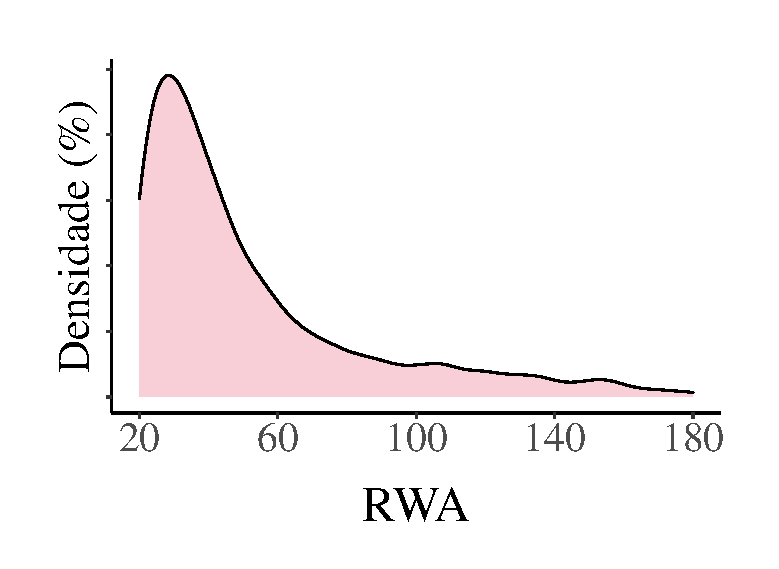
\includegraphics[width=1\linewidth]{figures/distribuicao_rwa}
		
		Fonte: \citeonline{open2016rwa}
	\end{minipage}
	\hspace{.05\linewidth}
	\begin{minipage}[b]{0.4\textwidth}
		\caption{Distribuição do Índice de Pós-Materialismo}
		\label{fig:pos_mat}
		\centering
		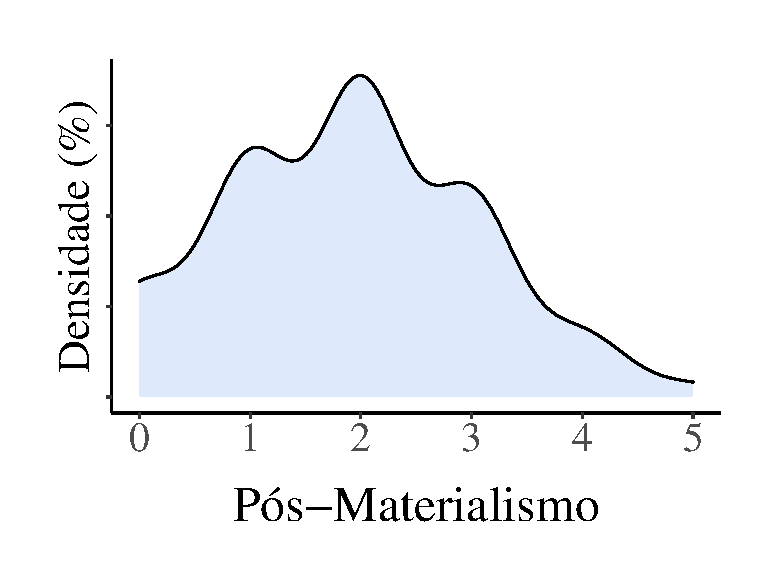
\includegraphics[width=1\linewidth]{figures/pos_materialism_index}
		
		Fonte: \citeonline{wvs2014wave}
	\end{minipage}
\end{figure}

Como efeito da sobreposição de elementos associados a confiança, tolerência e percepção de insegurança, o radicalismo ideológico associado ao RWA possui uma ocorrência esparça na população. Nas Figuras 1 e 2 é possível comparar a distribuição da escala com o Índice de Pós-Materialismo, proposto por \citeonline{inglehart2005modernization} e reconhecido como um indicador preciso de comportamentos liberais e pró-democráticos. Os dados sugerem que indivíduos com valores elevados para RWA estão longes do ponto mediano e, por isso, formam uma bolha atitudinal diferente do que observamos com indivíduos com baixos valores para Pós-Materialismo.

A existência de bolhas autoritárias na população tem efeitos significativos sobre a manutenção e replicação de movimentos radicais, os quais foram explorados em artigos sobre o tema. Além da maior imunidade em relação a formas distintas de pensamento -- lembre-se que o eleitor mediano e as propostas que visam-no estão distantes das faixas mais autoritárias -- essa parcela do eleitorado é facilmente mobilizável por \emph{outsiders} ou segmentos de representação dispostos a capturar suas intenções \cite{norris2017western, alexander2017myth}.  

De fato, em termos de dinâmica eleitoral, expera-se que a relação entre eleitores e representantes autoritários seja muito mais orgânica do que a interação convencional. Regimes autoritários podem angariar grande apoio popular, se uma parcela consistente da população percebe as restrição às liberdades como uma medida necessária contra ameaças e valida as fontes de informação do governo \cite{geddes1989sources, stein2013unraveling}. Portanto, é intutitivo concluir que a natureza da representação política para indivíduos autoritários é marcada por fortes traços delegativos.

\section{O discurso autoritário}

O discurso é um exercício de poder. É por meio da linguagem que registramos conhecimento, leis e regras de comportamento. Estes, por sua vez, compõem as principais categorias que humanos utilizam como referencial para interpretar o mundo ao seu redor. Por exemplo, se observamos alguém furar uma fila, julgamos sua atitude como justa ou oportunista, legal ou criminosa e moral ou anti-ética. Esses termos estão diretamente conectados a instituições sociais como o Estado e a Religião. 

Contudo, é importante ressaltar que, apesar dos grandes enunciados que constituem nossos guias de comportamento estarem ancorados na crença coletiva de sua validade, a capacidade de instituí-los está concentrada em poucos indivíduos \cite{foucault1969archeologie}. Ou seja, populações creditam legitimidade às suas leis e religiões, porém apenas uma pequena parte da nação é capaz de exercer influência direta no conteúdo de constituições e ritos.

A existência de um ranking social, que possui lugar de destaque para poucos e de subalternidade, para muitos, possui gênese anterior a civilização como conhecemos. As assimetrias que observamos nas relações sociais são fruto de um longo histórico de disputas e competição que acompanham a trajetória de sobrevivência de todas as espécies. Nessa dinâmica, a subserviência pode ou não ser conquistada por meio da força, mas sua manutenção se dá de maneira pacífica, na medida em que é naturalizada. 

Dentre as causas da hierarquia entre indivíduos, que funda a desigualdade observada na comunicação, a literatura aponta características individuais como determinantes significativos do desenvolvimento de dominância em grupos animais e humanos. Pesquisas documentam cor \cite{bakker1983determinants}, idade \cite{cote2000dominance, bohlin2001determinants}, peso corporal \cite{morgan2000predictors}, altura \cite{huang2002camera} e aparência \cite{lawson2010looking, lodge2013rationalizing} como alguns dos preditores da posição social de um indivíduo.    

Se por um lado características individuais explicam o surgimento da dominância, por outro, não são o único ingrediente do surgimento e estabilidade de cadeias de hierarquia que envolvem muitos integrantes. A disputa pelo lugar de dominância é mediada pela dinâmica interna dos grupos que compõem uma sociedade \cite{ridgeway1989dominance} e, em seguida, das relações entre os grupos \cite{chase1980social,chase2002individual}. Ou seja, a desigualdade é segmentada por clivagens formadas a partir de uma dinâmica complexa que envolvem aglutinações hierarquizadas de individúos em grupos que podem ser ordenados por status.  

Como argumentam \citeonline{sidanius2001social}, uma vez que grupos sociais são formados em torno de clivagens específicas -- por exemplo idade, gênero, clãs, nacionalidade, religião, cor e classe social -- seus integrantes reproduzem comportamento competitivo no qual buscam estabelecer superioridade. Nessa dinâmica, a formação de grupos dominantes e dominados estabelece a base da desigualdade, que consiste em uma sobreatribuição de valores positivos aos dominantes e, de valores negativos, aos dominados. Dado que discursos refletem relações de dominância presentes na sociedade, expressões linguísticas do autoritarismo tendem a carregar traços valorativos presentes no seu conteúdo ideológico: a exaltação das figuras reconhecidas como autoridade e a depreciação de grupos minoritários de status social mais baixo. 

Isto posto, o autoritarismo pode ser lido como uma propriedade que emerge de sistemas sociais desiguais e hierarquizados, nos quais a dominância é reafirmada como narrativa política. Conforme argumentou-se na seção anterior, indivíduos autoritários aprensentam maior propensão a expressão de preconceito e discriminação em geral. Ainda sobre o conteúdo de discursos autoritários, a literatura aponta a conexão entre autoritarismo e demonstração de hostilidade \cite{siegel1956relationship} e trabalhos que se dedicaram a investigar grupos políticos extremistas produziram resultados que sugerem que o dogmatismo político está correlacionado ao uso de discurso de ódio contra adversários e minorias \cite{gerstenfeld2003hate, ben2016hate}.  

O discurso autoritário apresenta ainda dimensões revelevantes no que dizem respeito a sua forma e estilo. \citeonline{beauzamy2013discontinuities} argumentou que dois traços comuns ao discurso facista no passado e no presente, são: i) o uso de argumentos elaborados com base em pseudo-ciência, teorias da conspiração, considerações mágicas e exegese religiosa e ii) uso de clichês e esteriótipos populares como metáforas em menções pejorativas a populações marginalizadas. Numa investigação similar, \citeonline{khany2014systemic} analisaram 20 discursos de personalidades históricas como Hitler, Stalin e Gadhafi. Como características comuns, apontaram a i) o majoritarismo e a massificação, ii) a defesa da incorruptibilidade do governo e iii) a manipulação das expectativas da opinião pública.

Em convergência com essa caracterização, \citeonline{smith1990symptomology} apresentou constribuição relevante para uma tipologia dos discursos autoritários analisando debates parlamentares acerca da ``proibição do fomento a homosexualidade'', que ocorreram entre as décadas de 80 e 90, nos EUA. Segundo a autora as falas autoritárias que emergiram sobre o tema apresentavam um traço marcante: a evocação de preconceitos e associações espúrias como método de enquadrar a discussão de forma desfavorável para a população gay. Em um dos exemplos dessa atitude, a menção à soropositividade como \emph{link} entre homossexualidade e problemas de saúde pública:

\begin{quote}
	A hegemonic interpretation of the AIDS phenomenon is, for example, actually a representation of radical difference, situated within a long tradition of similar representations of 'other' social elements. This AIDS discourse is linked genealogically to popular anxieties about various diseases, communist infiltration, immigrant populations, crime 'waves', drug 'crazes', etc. \cite{smith2015advances}
\end{quote}

A conexão entre soropositividade e homossexualidade é um caso típico do fenômeno cognitivo documentado como \emph{illusory correlation}, segundo o qual duas categorias de eventos são associadas sem que sua co-ocorrência estatística seja signficativa. Além de uma inferência incorreta, capaz de estimular conclusões inadequadas, está na raiz do reforço de esteriótipos de raça, gênero e sexualidade que fazem parte do discurso autoritário. Quando indivíduos percebem maior frequencia relativa de comportamentos rejeitados em um grupo, há uma tendência de identificá-los como atributo intrínseco ao grupo em questão, mesmo que a ocorrência absoluta de ``imposturas'' seja baixa \cite{sidanius2001social}.   

Além da frequente expressão de rejeição às populações identicadas como desviantes, discursos autoritários também envolvem constantes apelos a restauração da autoridade. Narrativas organicamente conectadas com o passado, que proclamam a restauração da ordem social e dos bons tempos que precederam o período atual tendem a ser instrumento de políticos autoritários para se colocarem como alternativas de crise \cite{pinto2004indoctrinating, mietzner2014indonesia}. 

Com isso, políticos autoritários as vezes se apresentam como alternativas radicais para condução de processos revolucionários ou de transição radical. Nesses cenários, discursos populistas que antagonizam as elites no poder com o ``verdadeiro povo'' são a principal estratégia eleitoral lideranças \cite{muller2017populism, levitsky2018democracies}. A ploclamação de uma conexão íntima com a cultura, a tradição e os anseios da massa e o uso de forma verbal imperativa, autocentrada e reativa também são características marcantes de figuras autoritárias que buscam estabelecer uma nova hegemonia \cite{goldschlager1982towards, gounari2018authoritarianism, hunter2019bolsonaro}.

Em síntese, o discurso autoritário é marcado por forte traço de polarização entre autoridades e indivíduos desviantes. Seja por referência direta ou indireta, às autoridades são atribuídas fortuna moral e, aos deviantes, todo o mal experienciado pelos "verdadeiros cidadãos". De modo a cristalizar valores e dogmas, políticos autoritários frequentemente apelam para falas majoritaristas que relembram o passado de maneira nostálgica e ascentuam as ameaças do presente. Como solução, apresentam-se em falas imperativas e hierarquizadas como guias para retomada da ordem e segurança. 


\chapter{Como classificar Agentes Autoritários?}\label{metodologia}

\section{As estratégias convencionais}

Conforme foi apresentado na seção \emph{Autoritarismo na política}, no capítulo 2, diversos trabalhos em Ciência Política se dedicaram a identificar causas e efeitos de políticos autoritários em regimes democráticos. Para isso, utilizam-se de um conjunto de estratégias metodológicas para classificar um agente autoritário. Nesse capítulo, abordará-se os principais critérios de classificação da literatura.

\subsection{Avaliação de Especialista}

A primeira e mais popular forma de classificação baseia-se em estudos de caso de lideranças políticas, nos quais suas atitudes e comportamentos são observados a partir de pronunciamentos, discursos e presença na mídia. A partir daí, são analisados holísticamente, tomando como base um referencial teórico, e, então, são identificados ou não como autoritários.

Alguns dos exemplos dessa abordagem podem ser encontrados nos trabalhos de \citeonline{seligson2003democracies}, \citeonline{seligson2005feeding}, \citeonline{weyland2013latin} e \citeonline{levitsky2018democracies}. Em cada um deles, as autoras e os autores identificam características nas lideranças políticas -- em geral chefes do executivo -- que sugerem comportamento anti-democrático. Em algum dos casos, como o de Chavez, na Venezuela, e do General Hugo Banzer, na Bolívia, atos realizados após o início dos seus governos também fazem parte do escopo de análise.

Entre as vantagens desse modelo de classificação, a precisão certamente é a principal delas. Construindo uma narrativa com tantos elementos, a credibilidade das suas conclusões é elevada. Pesquisas que optam por realizarem estudo de casos de líderes costumam oferecer um conjunto rico e convincente de evidências para seus resultados.

Apesar da precisão na identificação, a abordagem baseada na análise de especialistas apresenta grandes limitações. Como trata-se de uma extensa coleta de informações sobre um agente político -- não raramente realizada de forma não sistemática -- a capacidade de replicabilidade dessas pesquisas é baixa e sua abrangência é limitada. Como recursos de pesquisa são limitados, líderes autoritários tendem a ganhar espaço nessas investigações acadêmicas apenas após ascenção para lugares de poder nos quais já representam risco para o regime demcorático.

\subsection{Análise de Movimento Político}

Nas investigações da dinâmica eleitoral de movimentos autoritários em regimes democráticos, partidos políticos frequentemente são tomados como unidade de análise, porém movimentos sociais também integram essas análises \cite{caiani2017radical}. Como efeito, a literatura conta com um extenso histórico de pesquisas e registros que identificam a evolução desses partidos e grupos organizados ao longo da história recente, tanto no que diz respeito a desempenho como radicalização \cite{norris2005radical, mudde2009populist, caiani2017radical, mudde2016introduction, mudde2017ideational}. 

Como critério de clasificação de partidos autoritários, a Análise de Agenda Partidária baseia-se na ideologia expressa diretamente pelos partidos, em manifestos e programas de governo, na percepção do eleitorado da sua posição no espectro político, e das suas raízes históricas \cite{mudde2000ideology}. Frequentemente \emph{surveis} com o eleitorado também integram fonte de informação para o enquadramento em tipologias \cite{booth1984political, booth1994paths, macwilliams2016decides}. Como as unidades de análise estão presentes em pequeno número, ou são mensuradas de informa indireta, há, atualmente, uma grande cobertura no mapeamento realizado por pesquisadores independentes.

Um conjunto de trabalhos, que exemplifica essa abordagem, pode ser encontrada na literatura que trata de partidos políticos que herdaram, na sua fundação, recursos, conexões e ideologia dos governos autoritários que precederam as transições democráticas na América Latina \cite{loxton2015authoritarian, loxton2014authoritarian, lyons2016victorious, loxton2015authoritarian} e Europa Central \cite{grzymala2006authoritarian}. 

Nessas pesquisas, a construção de uma imagem de campanha baseada em uma extensa lista de referências aos signos militares, além forte conexão dos programas de governo com plataformas securitárias e anti-comunistas, compõem o critério de demarcação. Contudo, como esclarece \citeonline{mudde2000ideology}, investigar o fenômeno do autoritarismo, a partir de uma definição ideológica, possui uma limitação no que diz respeito a falácia ecológica:

\begin{samepage}
	\begin{quote}
		Although party ideology is said to be the most important criterion for classification, it is used only in an indirect way, i.e. through the eyes of the party itself (party name) or of the voters. \cite{mudde2000ideology}
	\end{quote}
\end{samepage}

Se por um lado é possível construir uma medida com grande cobertura e relativa precisão -- apesar discordâncias na classificação serem tema de discussões recentes da literatura \cite{glasius2018authoritarianism, mudde2016introduction} -- por outro há uma limitação no que diz respeito a profundidade das inferências baseadas em agentes políticos agregados.

\vspace{2cm}

\subsection{Survey com Elites}

A utilização de dados fruto de questionários aplicados a elites está presente no histórico de produções em Ciência Política\cite{hoffmann2007methods, andreadis2017elite}. Em consonância com a convergência recente da literatura para apontar papel preponderante das elites na formação da opinião pública \cite{zaller1992nature, gabel2007estimating, achen2017democracy}, essa abordagem é capaz de identificar o núcleo dos principais agentes de constuição e fomento de ideologias políticas.

A literatura que trata sobre populismo é um dos exemplos recentes de uso da técnica. Trabalhos como o de \citeonline{stavrakakis2017new} e \citeonline{andreadis2017european} dedicaram-se a utilizar respostas de \emph{surveis} aplicados a parlamentares para operacionalizar critérios de classificação de partidos populistas e mensurar a organicidade do vínculo entre representantes e eleitorado populista. Além disso, \citeonline{stevens2006authoritarian} dedicaram-se a identificar componentes da dinâmica autoritária entre elites políticas e civis -- no caso, a percepção de ameça e o apoio a soluções anti-democráticas.

Como argumenta \citeonline{ruth2015measuring}, a ferramenta de \emph{survey} permite a coleta de dados atitudinais de um universo maior de indivíduos que ocupam lugar de poder em governos. Parlamentares compõem uma peça importante em governos e na formação da opinião pública, porém permanecem inexplorados pela literatura. Devido às limitações das técnicas de análise de discurso, estudos de caso e entrevistas com eleitores em i) produzir resultados para grande número de casos ou ii) medir com precisão a ideologia política das elites políticas, uma parte importante da dinâmica populista permanece desconhecida. 

A posição de \citeonline{ruth2015measuring} pode ser facilmente estendida para o campo de estudos sobre autoritarismo. As técnicas revisadas ao longo desse cápitulo possuem limitações semelhantes às tratadas pelo autor e, consequentemente, as conclusões no que diz respeito a lacunas no conhecimento sobre autoritarismo entre parlamentares permanecem válidas. 

Todavia, \emph{survey} com elites possuem graves limitações. Um dos grandes impeditivos de sua execução é o acesso restrito a população de entrevistados. Como consequência, a periodicidade de bases de dados de atitudes políticas de parlamentares costuma ser baixa. Mesmo em iniciativas como o \emph{Comparative Candidate Survey} (CCS), que reune dados de questionários aplicados a candidatos e políticos em exercício de diversos países, possuem itens limitados no que diz respeito a mensuração da indicadores da personalidade autoritária. 

Como consequência das limitações, foram identificados apenas dois trabalhos nos quais autoritarismo foi mensurado direta ou indiretamente entre parlamentares por meio de \emph{survey} -- \citeonline{stevens2006authoritarian} e \citeonline{joly2018personality} são os únicos representantes da abordagem encontrados na revisão bibliográfica dessa dissertação. 


\section{Análise Automatizada de Conteúdo}

\subsection{O Estado da Arte da Análise Automatizada de Conteúdo}

Diante das limitações das abordagens anteriores, estratégias metodológicas que fazem uso de artefatos computacionais para otimizar processos de classificação têm se apresentado como uma solução para identificação em larga escala de atitudes e comportamentos de agentes políticos. Em particular, a literatura em Ciência Política que faz uso de Análise Automatizada de Conteúdo tem expandido seu escopo para ganhar aplicações em i) extração de informação sobre etnicidade a partir de nome \cite{roberts2016introduction}, ii) identificação de saliência temática em discursos de parlamentares \cite{batista2016mensurando, moreira2016palavra}, iii) construção de variáveis baseadas em componentes textuais \cite{curini2015conditional} e iv) extração de posicionamento ideológico implícito \cite{slapin2008scaling, ceron2016first}.

Os principais trabalhos de referência para classificação de parlamentares baseado em discursos concentram-se no campo de estudos sobre populismo. A partir de técnicas de codificiação baseadas em dicionário de termos, algoritmos de foram capazes de replicar, com relativa precisão e elevada escalabilidade, a classificação realizada por codificadores individuais de discursos populistas \cite{pauwels2011measuring, rooduijn2011measuring, oliver2016rise}. De forma similar, outras investigações utilizaram processamento de linguagem natural para automatização de partes do processo de identificação, como o reconhecimento de entidades associadas a adjetivos populistas \cite{kyle2018populists} e detecção de \emph{triplets} -- tríades compostas por sujeito, verbo e predicado \cite{aslanidis2018measuring}.

Para além da classificação de atributos atitudinais, algoritmos de aprendizado de máquina também têm sido capazes de modelar fenômenos psicológicos complexos como discurso de ódio \cite{davidson2017automated, zampieri2019predicting}, hostilidade \cite{hopp2017does, vargo2017socioeconomic, liu2018forecasting}, agressividade \cite{orasan2018aggressive, sahay2018detecting, nikhil2018lstms} e depressão \cite{mowery2016identifying, chekroud2016cross, orabi2018deep}. Esses resultados sugerem que há grande extensibilidade das aplicações, inclusive no que diz respeito a \emph{features} psicossocionais complexas, dentre elas, a personalidade autoritária.

Outra vantagem das ténicas de análise automatizada de conteúdo são sua grande versatilidade em termos de fontes e unidades de análise. A literatura angaria grande número de aplicações em \emph{big data} provenientes de Redes Sociais, \emph{blogs}, documentos oficiais e, no que diz respeito a Ciência Política, discursos, pronunciamentos e manifestos partidários \cite{grimmer2013text, wilkerson2017large, gentzkow2019text}. A escrita registra boa parte da atividade de agentes políticos, tanto dentro como fora do plenário. Uma vez que a comunicação é uma das principais formas de exercício de uma mandato e meio orgânico de \emph{accountability}, espera-se grande potencialidade dessa abordagem.

Todavia, algumas ressalvas importantes quanto a natureza dos modelos estatísticos de texto precisam ser salientadas. \citeonline{grimmer2013text} apresentou os \emph{4 Princípios da Análise Quantitativa de Texto}, são eles:

\begin{itemize}
	\item All quantitative models of language are wrong–but some are useful.
	\item Quantitative methods for text amplify resources and augment humans.
	\item There is no globally best method for automated text analysis.
	\item Validate, Validate, Validate.
\end{itemize}

Os tópicos sintetizam as maiores dificuldades da literatura que consome as novas técnicas de processamento de texto. Primeiramente, há grande perda de informação do valor semântico das palavras e frases quando elas são transformadas em dados de entrada em modelo estatístico. O sarcamo, por exemplo, é um recursos liguístico frequentemente utilizado para acentuar negativas, porém é elemento relativamente subidentificado por algoritmos de análise de conteúdo \cite{maynard2014cares}. Além disso, modelos de análise automatizada de conteúdo são significativamente sensíveis aos dados que recebem como \emph{input}. Amostras diferentes são capazes de produzir resultados significativamente distintos, mesmo que compartilhem mesma fonte.  

No que diz respeito ao desempenho e validação dos métodos, em artigo de \citeonline{dacrema2019we}, os autores abordaram o estado da arte dos algoritmos de recomendação. De 18 algoritmos considerados como representativos da literatura, apenas 7 foram capazes de ser replicadas de maneira apropriada e, desses, 6 apresentaram performance na revisão inferior a alternativas clássicas. Além de questionar os avanços gerados por implementações mais sofisticadas, o trabalho foi capaz de revelar graves limitações na reprodutibilidade e consistência no desempenho de técnicas de apredizado de máquina como um todo.  

Retomando o problema de pesquisa o qual esta dissertação busca resolver, de forma geral, avalia-se que o universo de \emph{Text as Data} apresenta uma saída consistente para a classificação de políticos autoritários. O potencial para processamento de grandes bancos de dados, com a possibilidade de modelar características individuais complexas, permite uma abordagem abrangente das atitudes de atores políticos cujo ofício implica no exercício da oratória.

Conforme argumentou-se no Capítulo 2, para lideranças autoritárias, discursos são ferramentas de mobilização do seu eleitorado cativo. Nas democracias contemporâneas, é por meio da fala, carregada de traços marcantes, que estes agentes políticos sedimentam e usufruem da dominância que estabelecem. A literatura converge para apontar que indivíduos dominantes tendem a utilizar mais tempo de fala e maior eloquência em seus discursos. Portanto espera-se que um parlamentar autoritário utilize com maior frequência seu espaço no plenário e, com isso, forneça dados suficientes para sua identificação e minimizar a ocorrência de falsos negativos. 

Autoritários silenciosos são tão raros quanto democratas no comando de ditaduras. 

\subsection{Propondo um novo Critério de Classificação}

Como forma de identificação alternativa de políticos autoritários, que possibilite a categorização em larga escala, de fomra ágil e generalizável, propõe-se um modelo baseado na análise automatizada de discursos e falas de agentes políticos. Atualmente, a comunicação política tem sido cada vez mais registrada em bancos de dados ou se proliferado em canais que possibilitam a coleta e armazenagem. Esse dado disponibiliza a operacionalização de técnicas que estimem atitudes políticas a partir de texto. Nos parágrafos a seguir, serão detalhados os passos e pressupostos dessa empreitada. 

Como ponto de partida, asume-se que discursos políticos se estruturam em torno de elementos e dimensões fundamentais, que retém uma parcela fundamental sobre seu sentido e significado. Ao longo de uma fala, parlamentares percorrem o Tempo -- que diz respeito tanto a um recurso limitado como a uma sequência linear em que frase se encadeiam -- e Temas -- que constituem agrupamentos amplos de setenças que as conectam em torno de um sentido. Dispostos em Tempo e Tema, estão 2 elementos fundamentais da comunicação: Entidades e Atributos. Enquanto Entidades são objetos linguísticos que podem ser nomeados -- como o sujeito de uma frase -- Atributos funcionam como descritores das Entidades -- como adjetivos e advérbios, uma vez que comportam valor de característica.

\begin{figure}[h]
	\caption{Diagrama do Discurso Político}
	\label{fig:discourse_representation}
	\centering
	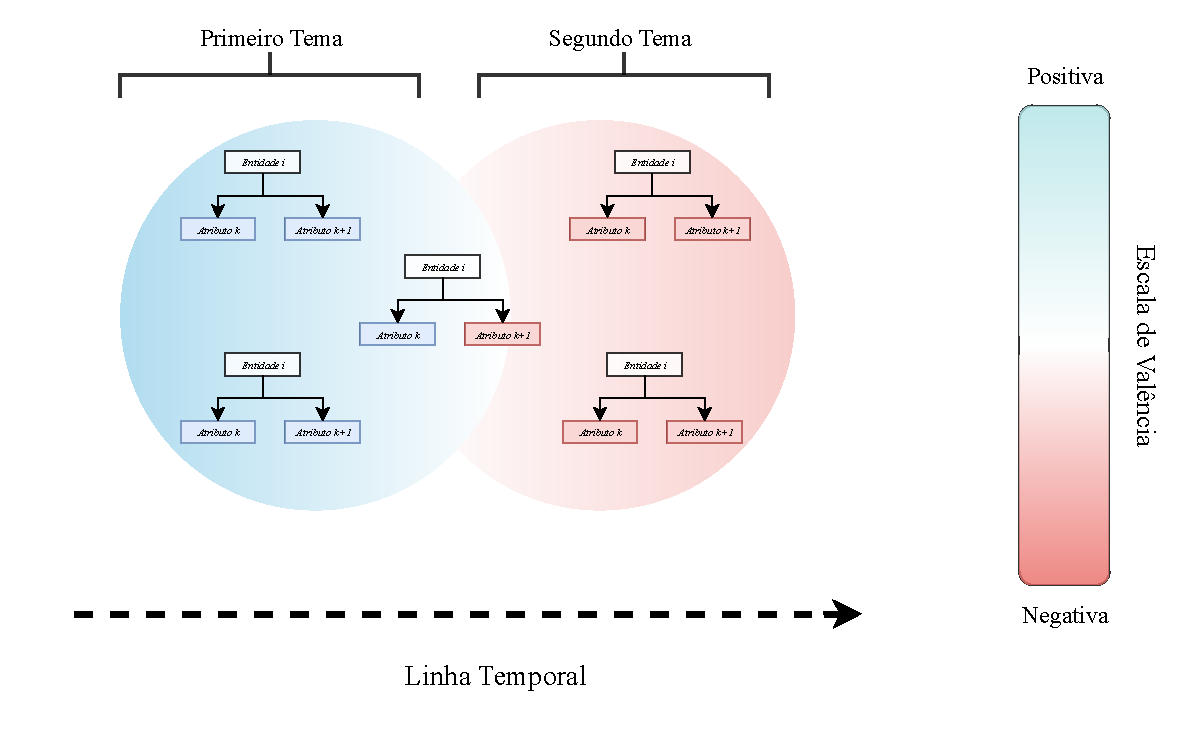
\includegraphics[width=1\linewidth]{figures/diagrama_discurso_autoritario}
	Fonte: elaboração do autor
\end{figure}

Figura 3 representa um diagrama simplicado do discurso político. A partir dele, pode-se compreender a dinâmica entre os elementos fundamentais e suas dimensões. Temas e Tempo ganham significado a medida em que um orador dispõem em sua fala setenças que conectam Atributos à Entidades. Uma vez que discursos políticos envolvem expressão de valor, espera-se que Atributos possuam uma polaridade -- positiva e negativa -- e que, por isso, funcionam como dispositivos para demarcar um posicionamento favorável ou desfavorável. Quanto mais Atributos negativos são utilizados para caracterizar as Entidades mencionadas sobre um tema, mais negativo será a compreensão geral da sentenças sobre o Tema.

Na Figura 3, as Entidades mencionadas no início do discurso tanto recebem atributos positivos como compartilham de uma atmosférica temática de maior valência. No outro extremo, as Entidades mencionadas ao final do discurso possuem o inverso dessas características -- Atributos e Tema e negativos. Portanto, pode-se inferir que, no escopo de Entidades do orador, seu posicionamento variou da simpatia manifesta no início da fala até a rejeição, ao final. Essa dinâmica discursiva remete ao caráter hierárquico da estrutura textual, na qual termos são unidades básicas da linguagem, sentenças concatenam sentido no nível local, e temas consolidam grandes conjuntos de expressão.    

Um exemplo prático dessa dinâmica está presente nas contribuições de \citeonline{smith1990symptomology}. Nas falas de parlamentares analisadas pela autora, a expressão de rejeição à minorias apresentou dois modos típicos: i) a atribuição direta de características negativas e ii) o estabelecimento de uma correlação ilusória a partir da menção de Entidades em Temas carregados de polaridade negativa -- como crime, entorpecentes e problemas de incivilidade. Do ponto de vista dos ouvintes, um grupo social que compartilha um mesmo espaço semântico que elementos popularmente reprovados também é passível de estigma. De forma simétrica, a exaltação de Entidades associadas às autoridades se dá pelos mesmos mecanismos.

Além do uso de Atributos, a posição em relação a uma Entidade é fortemente marcada pela frequência em que é mencionada nas falas de um agente. A saliência temática demarca tanto clivagens políticas como espaços de embate, uma vez que, no contexto de recursos limitados, é o principal indicativo de quais são as questões prioritárias. A recorrência na menção de uma pauta ou maior investimento de tempo de fala em discursos nos quais é mencionada eleva a magnitude das opiniões mobilizadas em torno dela e é determinante da ideologia do orador.

É intuitivo assumir, ainda, que Entidades, Atributos e Temas são elementos que se combinam de forma complexa em discursos politizados com o propósito de expressar conteúdo ideológico. Ou seja, é possível utilizar informação da fala dos oradores para inferir posicionamentos latentes e, no caso deste trabalho, estimar seus níveis de RWA. Para isso, assume-se que a Valência expressa em relação a certas classes de Entidade pode ser traduzida em adesão à grupos dominantes -- polaridade positiva -- e rejeição à grupos dominados -- polaridade negativa.

No Quadro 1 é possível observar uma tipologia de Entidades baseda na escala original proposta por \citeonline{altemeyer2006authoritarians} e nas versões brasileiras das escalas de RWA e F, adaptadas respectivamente por \citeonline{vilanova2018adaptaccao} e \citeonline{de2018analises}. As divisões do quadro correspondem aos Componentes que Integram a Escala RWA, aos Valores que representam dimensões específicas nas quais cada componentes se manifesta. As Raízes são porções genéricas de palavras, sem prefixo, sufixos e conjugações, e no quadro elas identificam as principais Entidades que representativas de cada Valor. Para definí-las, tomou-se como base o trabalho realizado por \citeonline{moreira2016palavra}, que mapeou os tópicos constitutivos do debate político brasileiro a partir do resultado de \textit{expressed agenda model} e dados textuais de pronunciamento parlamentares.  

\begin{center}
	Quadro 1 - Tipologia de Entidades
	
	\vspace{0.4cm}
	
	\begin{tabular}{llc}
		\toprule
{Componente}								& {Valor} 					& {Raízes} \\ \midrule
\multirow{2}{*}{Submissão à Autoridade} 	& Ufanismo				& \textit{brasil}, \textit{patri}, \textit{nação}, \textit{herói} \\
& Radicalismo Religioso		& \textit{deus},\textit{igreja},\textit{evangelic},\textit{catolic},\textit{crist},\textit{crent} \\ \midrule
\multirow{3}{*}{Agressividade Autoritária} 	& Punitivismo 				& \textit{polic}, \textit{seguranc}, \textit{milit}, \textit{exercit}, \textit{forcas} \\
& Patriarcalismo	 		& \textit{famil}, \textit{tradic}, \textit{home} \\
& Rejeição à Diversidade	& \textit{negr},\textit{racial},\textit{homossex},\textit{lesb},\textit{human},\textit{indigen},\textit{mulh} \\ \midrule
\multirow{3}{*}{Convencionalismo} 			& Majoritarismo 			& \textit{povo}, \textit{nós}, \textit{cidad}\\
& Hierarquia				& \textit{autorid}, \textit{trabalh}, \textit{empreg}, \textit{banc}, \textit{financeir} \\
& Anti-cientificismo		& \textit{estud}, \textit{univers}, \textit{pesquis}, \textit{cienc}, \textit{cient}, \textit{tecno} \\ \bottomrule
	\end{tabular}
	
	\vspace{0.6cm}
	
	Fonte: elaboração do autor com dados de \citeonline{moreira2016palavra} 
\end{center}

No contexto brasileiro, Ufanismo, Majoritarismo e Punitivismo são elementos centrais da narrativa que saúda o passado e propõem uma saída centralizadora e monotônica, que se utiliza do militarismo, para restauração. Entre os questionários originais e adaptados, estão presentes fortes referências a salvação do país por meio de punição mais rígidas e laços mais entreitos entre Estado e Sociedade Civil. Alguns dos exemplos são:

\begin{quote}
	1. Do jeito que as coisas estão indo nesse país, serão necessárias medidas severas para endireitar os meliantes, os criminosos e os pervertidos.
	
	2. A situação do nosso país está ficando tão séria que ações firmes seriam justificadas se eliminassem os desordeiros e nos levassem de volta ao nosso verdadeiro caminho.
	
	6. O que o nosso país realmente precisa é uma dose forte e dura de lei e ordem.
	
	29. Nosso país será melhor se obedecermos nossos líderes.
	
	34. Nosso país será melhor se mostrarmos respeito à autoridade.
	
	3. Não há nada pior do que uma pessoa que não sente profundo amor, gratidão e respeito por seus pais
	
	\cite{vilanova2018adaptaccao, de2018analises}
	
\end{quote}  

Além de aspectos políticos, também é possível observar uma dimensão associada a atitudes e comportamentos captada pelos valores de Radicalismo Religioso, Patriarcalismo e Rejeição à Diversidade. Cada um dispõe de um conjunto próprio de julgamentos que segmentam a população entre ``bons'' e ``maus'', oferecendo as bases para discriminação e intolerância contra grupos vulneráveis, minorias e indivíduos que questionam a autoridade e a tradição. É possível visualizar alguns desses elementos normativos a partir das afirmativas:
 
\begin{quote}
	
	15. As pessoas devem estar prontas para desafiar leis com as quais elas não concordam.
	
	
	18. As pessoas deveriam ter as suas próprias preferências sexuais, mesmo se isso torná-las diferentes do resto da sociedade.
	
	19. Não há nada de errado com sexo antes do casamento.
	
	21. As pessoas deveriam ter os seus próprios estilos de vida mesmo se isso torná-las diferentes do resto da sociedade.
	
	24. As leis de Deus sobre aborto, pornografia e casamento devem ser seguidas à risca antes que seja tarde demais.
	
	6. Todos devemos ter fé absoluta em um poder sobrenatural, cujas decisões devemos acatar.
	
	10. Os homossexuais são quase criminosos e deveriam receber um castigo severo.
	
	\cite{vilanova2018adaptaccao, de2018analises}
	
\end{quote}

Por fim, a Hierarquia e Anti-cientificismo celam um bloqueio triplo contra as principais fontes de contestação na sociedade: aqueles que não ocupam a posição de poder e aqueles que produzem novos conhecimentos. Autoritários tendem rejeitar contestações a suas crenças e apregam-se veementemente aos papeis sociais tradicionais, naturalizando a desigualdade. Buscando identificar esse tipo de disposição, os questionários incluem as afirmativas:
 
\begin{quote}
	
	16. Estudantes de colégios e universidades devem ser encorajados a desafiar, criticar e confrontar autoridades.
	
	13. A ciência tem o seu lugar, mas há muitas coisas importantes que a mente humana jamais poderá compreender.
	
	14. Os homens podem ser divididos  em duas classes definidas:  os fracos e os fortes.
	
	16. Pobreza é consequência da falta de vontade de querer trabalhar.
	
	\cite{vilanova2018adaptaccao, de2018analises}
	
\end{quote}

Como forma de mensurar o RWA a partir das falas de agentes políticos, tomou-se a expressão direta -- a nível de sentença -- e indireta -- a nível de contexto -- de adesão a cada um desses valores como indicativo de maior afinidade ao autoritarismo. A essa medida de propensão, deu-se o nome de escala de Valores Autoritários.

A Equação 3.1 especifica a estimação de expressão direta. Dado um Valor $v$, que compõem uma das dimensões do RWA, a adesão de um agente político se expressa pela razão da diferença entre o número de sentenças positivas -- $Pos_v$ --  e o número de sentenças negativas -- $Neg_v$ -- que mencionam alguma das Raízes que compõem a tipologia de Entidades no Quadro 1 e o número de sentenças de sentimento mais frequente -- $Pos_v$ ou $Neg_v$.

\begin{equation}
\beta_v = 
\begin{cases}
\frac{Pos_v - Neg_v}{Pos_v}, & \text{se}\ Pos > Neg \\
\frac{Pos_v - Neg_v}{Neg_v}, & \text{caso contrário.}
\end{cases}
\end{equation}

A Equação 3.2 especifica a estimação de expressão indireta. Dado o contexto do Discurso $k$, em que Entidades que compõem uma das dimensões do RWA são mencionadas, a adesão indireta de um agente político se expressa pela razão da diferença entre o número de sentenças positivas -- $Pos_k$ --  e o número de sentenças negativas -- $Neg_k$ -- contidas no contexto e o número de sentenças de sentimento mais frequente -- $Pos_k$ ou $Neg_k$.

\begin{equation}
\gamma_k = 
\begin{cases}
\frac{Pos_k - Neg_k}{Pos_k}, & \text{se}\ Pos > Neg \\
\frac{Pos_k - Neg_k}{Neg_k}, & \text{caso contrário.}
\end{cases}
\end{equation}

As estimativas geradas pelas Equações 3.1 e 3.2 resultam em valores que pertencem ao intervalo $[-1, 1]$, em que quanto mais próximo de 1, maior a probabilidade de adesão a um dos Valores que compõem a escala de Valores Autoritários e, mais próximo de -1. menor a probabilidade de adesão. 

Por fim, o indicador final é composto pela soma ponderada das duas estimativas, especificada na Equação 3.3. A escala de adesão, representada por $\theta$, também varia no intervalo$[-1, 1]$. A Equação 3.4 representa a normalização do valor de $\theta$. Se um indivíduo possui resultante positiva, então apresenta algum nível de adesão ao valor autoritário e soma 1 ponto na Escala de Valores Autoritários. Como tratam-se de 8 Valores, a escala varia entre 0 -- rejeição de todos os Valores autoritários -- e 8 -- adesão à todos os valores autoritários.

\begin{equation}
\theta_{vk} = 0.75 * \beta_v +  0.25 * \gamma_k
\end{equation}

\begin{equation}
AuthVal_v = 
\begin{cases}
1, & \text{se}\ \theta_{vk} > 0 \\
0, & \text{caso contrário.}
\end{cases}
\end{equation}

Tomando um exemplo anedótico, para o valor de Punitivismo, um indivíduo que manifestou $\beta = 0.5$ -- portanto se inclinou diretamente ao Valor -- e $\gamma = -0.8$ -- inserindo a menção ao Valor em um contexto muito negativo -- apresenta $\theta = 0.175$ e, assim, recebe 1 ponto na escala de Valores Autoritários -- $AuthVal$. Para definir os pesos dos componentes de $\theta$, tomou-se como referência a literatura que trata de \emph{Social Desirability Bias}. Trabalhos que estimaram a subnotificação de compra de votos, xenofobia e racismo apresentaram resultados entre 20{\%} e 30{\%} \cite{rudmin1999norwegian,heerwig2009education,gonzalez2012vote}.

É necessário, contudo, lidar com um fator adicional. Como agentes políticos possuem agendas diferentes, é esperado que apenas uma parte dos oradores façam menção à todos os Valores da escala de Valores Autoritários, seja para manifestar adesão ou rejeição. Um parlamentar que possui pautas sanitárias como centro da sua representação, por exemplo, tende a se manifestar sobre questões punitivas com menor frequência. Como efeito, a escala apresenta viés de seleção e incorpora efeitos endógenos da saliência temática dos agentes políticos.

Como forma de aproximar a escala de Valores Autoritários de um indicador consistente de RWA, utilizou-se inferência bayesiana. Nesse sentido, a estimativa de RWA de um agente político é composta por uma porção de informação a priori, que envolve o que sabe-se sobre a distribuição de RWA na população, e uma porção de informação definida pela verossimilhança, que obtem-se a partir dos dados, decomposta pela escala de Valores Autoritários. 

Como informação a priori, assume-se que o RWA entre agentes políticos segue uma distribuição Poisson, tal como sugerem os dados coletados a partir de respostas para questionário original, como na Figura 1. Uma vez que foram delimitados 8 conjuntos de Valores, a distribuição pertence ao intervalo $[0, 8]$, de parâmetro $\lambda = 1.62$\footnote{O parâmetro $\lambda$ foi estimado a patir dos microdados de \citeonline{open2016rwa}. Para isso, tomou-se a média da escala de RWA dos respondentes que levaram até o quantil 95 de tempo para responder o questionário e que cometaram no máximo até 2 erros, de 16, nas questões de validação.}. Para inferir uma média de RWA para a população, basta calcular a esperança da distribuição ao longo de todo o intervalo, representada pela área A na Figura 4.

\begin{figure}[!htb]
	\caption{Distribuição Priori e Posteriori RWA}
	\centering
	\begin{minipage}[b]{0.4\textwidth}
		\textbf{Priori}
		\label{fig:rwa_area_total}
		\centering
		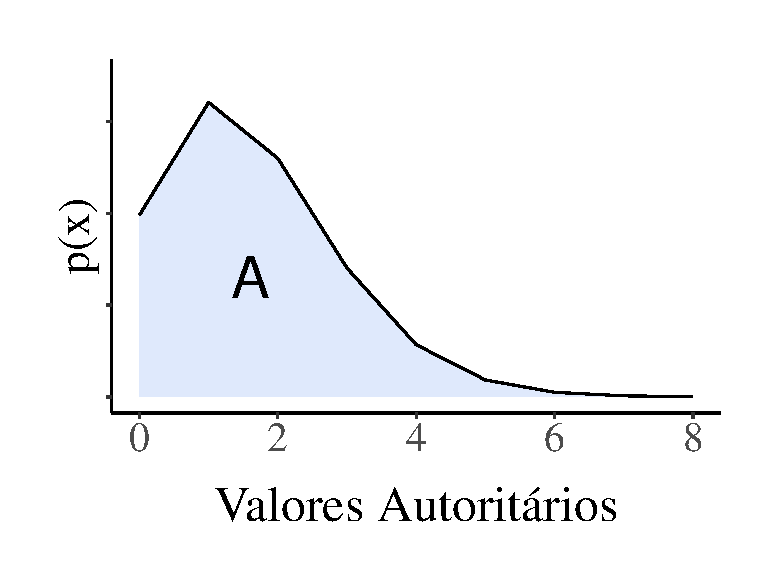
\includegraphics[width=1\linewidth]{figures/area_total_rwa}
			\end{minipage}
\\
	\hspace{.05\linewidth}
	\begin{minipage}[b]{0.4\textwidth}
		\textbf{Posteriori}
		\label{fig:rwa_area_min}
		\centering
		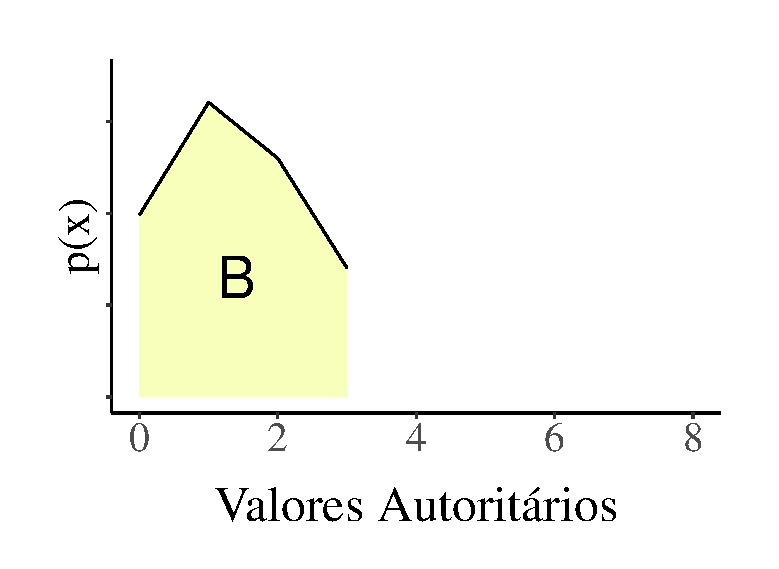
\includegraphics[width=1\linewidth]{figures/area_parcial_min_rwa}
		
	\end{minipage}
	\hspace{.05\linewidth}
\begin{minipage}[b]{0.4\textwidth}
	\textbf{Posteriori}
	\label{fig:rwa_area_max}
	\centering
	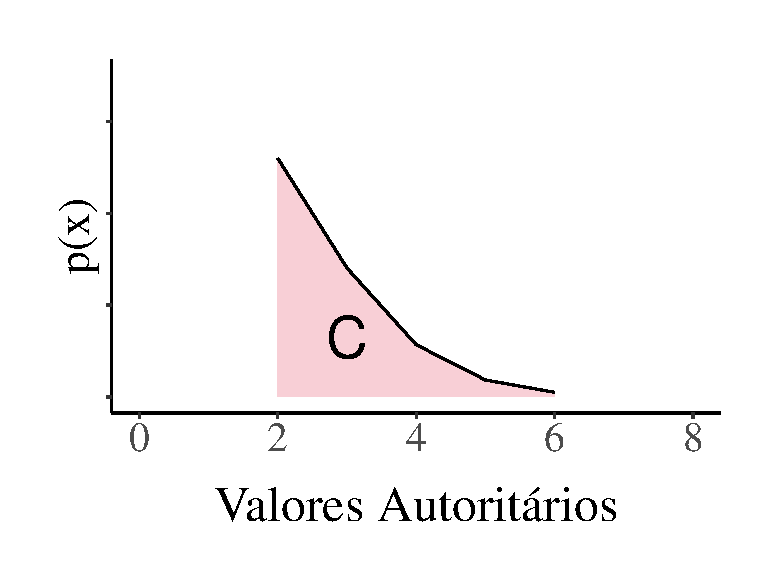
\includegraphics[width=1\linewidth]{figures/area_parcial_max_rwa}
	
\end{minipage}

Fonte: elaboração do autor
\end{figure}

Como ponto de partida, é intuitivo atribuir o valor médio a um agente político qualquer. Porém, na medida em que adquirimos mais informação, mensurando a escala de Valores Autoritários, é possível introduzir condicionais no cálculo da esperança, restringindo o espaço de eventos e conseguindo alcançar um valor médio que converge para um ponto mais preciso. 

Na Figura 4, na área B, também é possível visualizar o polígono resultante de um indivíduo que se manifestou sobre 5 dos 8 Valores e rejeitou todos. Como efeito, dois cenários extremos são possíveis, caso se manifestasse sobre os outros 3 Valores: rejeitar todos ou aderir a todos. Com isso, a aŕea que corresponde o espaço de eventos restringe ao polígono formado pela distribuição no intervalo $[0, 3]$. Já na área C, é possível visualizar a representação de um indivíduo que se manifestou sobre 4 Valores, aderiu a 2 deles e rejeitou outros 2. Nesse caso, os cenários extremos são: rejeitar os outros 4 e aderir a todos eles. Assim, o RWA estimado se retringe a esperança da distribuição no intervalo $[2, 6]$. Comparativamente, o valor de RWA estimado para os casos A, B e C são, respectivamente, 1.62, 1.37 e 2.68.

Alguns detaques importantes nos procedimentos de estimação são que a distribuição a priori, especificada na Equação 3.5 e visível na distribuição da área A, na Figura 4 resguarda os pressupostos de uma distribuição de probabilidade. Para que os polígonos gerados a partir da restrição de intervalos, como no caso das áreas B e C da Figura 4, contudo, é necessário atualizar os valores da variável aletória para que a integral da função de probabilidade resulte em 1, conforme especifica a função composta na Equação 3.6. 

A inclusão de num novo componente no denominador, que consiste na soma das probabilidades do valores que compõem o intervalo $[L, U]$, tem como efeito normalizar as probabilidades no polígono. Ou seja, a escala de Valores Autoritários entrega os parâmetros de \emph{upper bound} e \emph{lower bound}, utilizados para definir o espaço de eventos. Por fim, a Equação 3.7 especifica o cálculo da esperança da distribuição que tem como resultante o valor estimado de RWA e a Equação 3.8, a variância da estimativa. 
     

\begin{equation}
f(x) = \frac{\mathsf{e^{-\lambda}} \,\lambda^{x}}{x\,!}
\end{equation}

\begin{equation}
g \circ f(x,\, L, \,U) =\frac{\mathsf{e^{-\lambda}} \,\lambda^{x}}{x\,! \, \displaystyle\sum_{k = L}^{U} f(k)}
\end{equation}

\begin{equation} \label{eq1}
\begin{split}
\widehat{rwa} & = E(x) \\
E(x|L, U) & = \int_{L}^{U} g \circ f(x, L, U) \,x \,dx
\end{split}
\end{equation}

\begin{equation}
\begin{split}
\sigma^{2} & = E(x^{2}) \\
E(x^{2}|L, U) & = \int_{L}^{U} g \circ f(x, L, U) \,x^{2} \,dx
\end{split}
\end{equation}

É possível observar a proporcionalidade entre a quantidade de Valores Autoritários e o RWA estimado, porém os resultados obtidos por meio de atualização bayesiana apresentam correções contra subestimação e viés de seleção.

\subsection{Operacionalizando a Estimação dos Parâmetros}

Para estimarmos o valor de RWA de um agente político é necessário definir um método de mensuração da Valência das Sentenças associadas às Entidades. Conforme argumentou-se, a Valência é um componente que se expressa a nível de sentença e de contexto, manifestando a adesão e rejeição nas suas formas direta e indireta. É a partir do indicador de que uma sentença é positiva que pode-se calcular os parâmetros $\beta$ e $\gamma$ das Equações 3.1 e 3.2. E para definição do escopo do contexto, é necessário identificar a qual tópico ou tema a Entidade de interesse está inserida. Com as duas informações, é possível compor imagens como a Figura 3, que detalham a dinâmica discursiva de um discurso político.

Antes de detalhar a estratégia operacional é necessário caracterizar o uso da Valência como indicador de apoio e desaprovação. Para isso, é importante ressaltar que a validade de modelos baseados em dados textuais envolve a expectativa de que é possível estabelecer equivalência entre valores numéricos e emoções humanas. Além disso, todo modelo carrega um caráter de representação da realidade, que ganha precisão quanto mais for validada. Apesar de críticas que apontam que essas duas premissas são fortes demais para serem aceitas em pesquisas sobre comunicação política \cite{miguel2015vale}, a análise de valências têm se popularizado e conta com enorme respaudo acadêmico \cite{feres2016analise}.      

Como opção metodológica, adotou-se a Análise de Sentimentos, uma solução algorítmica para análise de textos, desenvolvida para extração e identificação de emoções, sentimentos e atitudes, altamente escalável. Ao longo das três últimas décadas, tem sido cada vez mais utilizada para a automatização no processamento de \emph{reviews} no mercado digital e extração de \emph{features} textuais de opinião pública. Quanto às premissas do modelo e o tipo de resposta que oferece, algoritmos dessa natureza partem do postulado de que toda sentença possui uma valência, ou seja, um posicionamento latente que pode ser tipificado em pró, contra ou neutro -- frequentemente assinalados com os valores -1,0 e 1 -- que representam as classes do \emph{target} na otimização do modelo \cite{serrano2015sentiment, mantyla2018evolution}.  

Uma das formas de calibrar o algoritmo consiste no uso de dicionários codificados, construídos a partir da classificação de termos e expressões que carregam carga semântica negativa ou positiva. Nesse sentido, alguns dos modelos propostos na literatura ancoram-se em artefatos produzidos no campo da linguística e psicologia para conectar palavras a sentimentos, inclusive com grande complexidade. Um desses exemplos é o PANAS-t, desenvolvido por  \citeonline{gonccalves2013panas}, que baseia-se na escala psicométrica PNAS, proposta por \citeonline{watson1988development} e posteriormente estendida por \citeonline{clark1994manual}. A escala, elaborada a partir de entrevistas nas quais respondentes descreviam como se sentiam em relação a certos eventos, identifica expressões associadas a afeição e rejeição. 

Anos antes, \citeonline{bollen2010determining} apresentaram um modelo baseado na escala POMS \cite{mcnair2003profile} que, partindo da mesma estratégia, identificava a valência de uma sentença a partir da frequencia relativa de suas palavras e suas correspondências como a tipologia estabelecida. Contudo, o estado da arte das estratégias baseadas em dicionários é ocupado por combinações de tipologias, uso de fontes mistas -- como \emph{emoticons} --  e processos generativos automatizados, como a interpolação da valência de uma palavra para seus sinônimos e tipificação baseada em coocorrência \cite{hogenboom2013exploiting, hutto2014vader, thelwall2014sentistrength, canuto2016exploiting}.

Uma alternativa às técnicas baseadas em dicionários são o modelos de \emph{Machine Learning} que tomam texto como \emph{features} na previsão de um \emph{target} que, nesse caso, é composto por classes de sentimentos\footnote{Do ponto de vista da implementação, as soluções mais simples prodecem da seguinte forma: 1) o texto é preprocessado, \emph{stopwords} e símbolos são removidos, 2) as palavras que compõem cada sentenção são divididas e as com menor frequência são retiradas 3) a partir de todas as palavras que compõem o banco de dados, sentenças são representadas por uma série de variáveis binárias que identificam a presença ou não de cada uma das palavras e 4) um modelo de regressão logística é treinado utilizando as variáveis binárias como variáveis independentes e o \emph{target}, como variável dependente. Soluções mais complexas envolvem métodos mais sofisticados de transformam das sentenças em variáveis numéricas -- como \emph{Word2Vec} -- e modelos mais adequados para lidar com multicolinearidade e otimização -- como \emph{Ensemble Learning}.}. O primeiro trabalho a adotar essa abordagem foi apresentado por \citeonline{pang2002thumbs} que, se utilizando de uma base de \emph{reviews} de produtos, tomou das \emph{n-grams} -- sequências contínuas de palavras -- das sentenças como \emph{inputs}. Atualmente, a literatura documenta modelos de elevado desempenho, que atingem grande precisão de classificação, mesmo como bases de treinamento rotuladas por não-especialistas \cite{howard2018universal, sun2019fine, yang2019xlnet}. Essa abordagem, contudo, implica em custos de elaboração e implementação significativamente caros, uma vez que imprescindem de codificação em larga escala e grande poder computacional para atingirem precisão satisfatória.

Para definição do modelo de classificação, relizou-se experimentos tomando os 4 principais dicionários léxicos de sentimentos para língua portuguesa: ReLi, LIWC, OpLexicon e SentiLex-PT. O ReLi concatena anotações de 1600 resenhas de 14 livros diferentes \cite{freitas2012vampiro, freitas2014sparkling} e foi transformado em léxico a partir do trabalho de \citeonline{freitas2013construccao} por meio da codificação de vocabulário afetivo. O LIWC é produto de uma investigação psicológica sobre a expressão de sentimentos de estados mentais por meio da linguagem que contou com aplicação extensa de questionários não-estruturados \cite{pennebaker1996cognitive, pennebaker1997linguistic}. Já o OpLexicon e SentiLex-PT se diferenciam das alternativas anteriores por utilizarem codificação automatizada na composição dos léxicos \cite{souza2011construction, carvalho2015sentilex}.

Quanto aos procedimentos realizados na etapa de preprocessamento do texto, as seguintes transformações são realizadas nas sentenças: i) eliminação de pontuação, símbolos e números; ii) remoção de \emph{stopwords} (artigos, preposições, conjunções ...); iii) conversão de todas as palavras da sentença para minúsculo. Vale ressaltar que as raízes das palavras não foram extraídas, uma vez que a flexão é relevante em classificações por dicionário léxico. Partindo da sentença preprocessada, para extração do sentimento, utilizou-se a regra de bolso adotada por \citeonline{gonccalves2013panas}, na qual as quantidades de termos positivos e negativos são relacionadas por meio da fórmula da Equação 3.9.

\begin{equation}
P(s) = 
\begin{cases}
\frac{\alpha_s - \beta_s}{\alpha_s}, & \text{se}\ \beta_s \leq \alpha_s \\
\frac{-1(\beta_s - \alpha_s)}{\beta_s}, & \text{se}\ \beta_s > \alpha_s
\end{cases}
\end{equation}

Sendo $P(s)$ a polaridade da sentença \emph{s}; $\alpha_s$ a quantidade de termos positivos na sentença e  $\beta_s$ a quantidade de termos negativos.

Como base de avaliação dos experimentos, utilizou-se um banco de dados, de elaboração própria, composto pelas setenças das 511 declarações de voto na sessão que discutiu a admissibilidade do \emph{impeachment} de Dilma Roussef. As sentenças foram codificadas manualmente em 3 categorias de valência: negativas, neutras e positivas. Uma vez que a sessão contou com grande audiência, num momento de intensas manifestações civis no país, as falas dos parlamentares manifestaram-se em um microcosmos de afetos políticos. Com isso, constitui-se um cenário ideal para mensurar a precisão de métodos de classificação de sentimentos.   

Para construção dos modelos, utilizou-se como referência o trabalho de \citeonline{machado2018creating}, os quais propõem estratégias de otimização no uso de dicionário léxicos em problemas de classificação\footnote{\citeonline{machado2018creating} definem estratégias que implicam em ganhos significativos de desempenho na classificação. A primeira delas consiste no uso de advérbios de negação como identificadores de pontos de inversão da valência de um atributo. Nos exemplos ``\textit{Não! Ele é honesto}'' e ``\textit{Ele \textbf{não} é honesto!}'', a referência a honestidade possui pesos opostos que são demarcados pela posição do termo 'não' na frase. Outra contribuição importante envolve os métodos de combinação de dicionários léxicos. Tanto nos experimentos realizados pelos autores como nos realizados neste trabalho, a opção por ordem de uso das predições implicou em resultados significativos diferentes.}. O desempenho de cada experimento pode ser visualizado na Tabela 1. As métricas de Precisão Ponderada e Recall Ponderado indicam que o ReLi possuiu melhor desempenho individual, porém a combinação das classificações geradas por ReLi, LIWC e OpLexicon apresentou os melhores resultados\footnote{A combinação toma a predição do LIWC para a classe negativa, a predição do ReLi para a classe neutra e do OpLexicon, para a positiva.}. O modelo adotado, com isso, apresenta métricas satisfatórias -- para uma classficação de 3 classes -- e assegura uma estimativa válida para a valência de falas proferidas por agentes políticos.   

\begin{center}
	Tabela 1 - Desempenho de Modelos de Classificação de Sentimentos
	
	\vspace{0.4cm}
	
	\begin{tabular}{lcc}
		\toprule
		{Léxicos}					& {Precisão Ponderada} 	& {Recall Ponderado} \\ \midrule
		{ReLi} 						& 0.54					& 0.58 \\ 
		{LIWC} 						& 0.58					& 0.47 \\ 
		{OpLexicon} 				& 0.53					& 0.50 \\ 
		{SentiLex} 					& 0.54					& 0.54 \\ 
		{ReLi + LIWC + OpLexicon} 	& 0.59					& 0.59 \\ 
		\bottomrule
	\end{tabular}
	
	\vspace{0.6cm}
	
	Fonte: elaboração do autor
\end{center}     

Mantendo a opção por técnicas de análise de conteúdo escaláveis e extensamente validadas, o LDA foi escolhido como método para definição do escopo dos contextos. Proposto por \citeonline{blei2003latent}, para identificação de tópicos, trata-se de um algorimto não-supervisionado -- que portanto não necessita ser especificado -- que toma documentos como o produto da geração de palavras por $k$ tópicos e possui como \emph{output} listas de termos representativos para cada conjunto. O LDA é bastante popular na literatura e conta com implementações para as ferramentas mais utilizadas pelas comunidade. Entre as premissas do modelo estão:

\begin{itemize}
	\item A distribuição da ocorrência de termos constitui uma variável latente para temas e tópicos em um texto.
	\item A frequência das palavras nas sentenças segue uma distribuição \emph{Poisson}, representada por pela variável aleatória $N$.
	\item A probabilidade associada ao pertecimento de um tópico está associado a uma variável aleatória de distribuição \emph{Dirichlet} de dimensão \emph{k}.
	\item Tópicos identificados no LDA possuem a propriedade estatística de permutabilidade, ou seja, são independentes entre si em cada documento. 
\end{itemize}

Como consequência do terceiro item, o LDA não se trata de um classificador de palavras, como cada tópico é independente dentro de cada documento, os temos gerados pelo algoritmo para compor cada um dos conjuntos de termos representativos, alguns deles podem estar presente em mais de um tópico. Todavia, uma estratégia simples para adaptar a técnica para fins de classificação é atribuir, a um trecho textual, o tópico com o qual compartilha mais termos. A partir daí, para mensurar a valência média de cada tópico, basta calcular a média da valência das sentenças de todos os trechos textuais associados.

\begin{figure}[h]
	\caption{Diagrama do Modelo Generativo no LDA}
	\label{fig:lda}
	\centering
	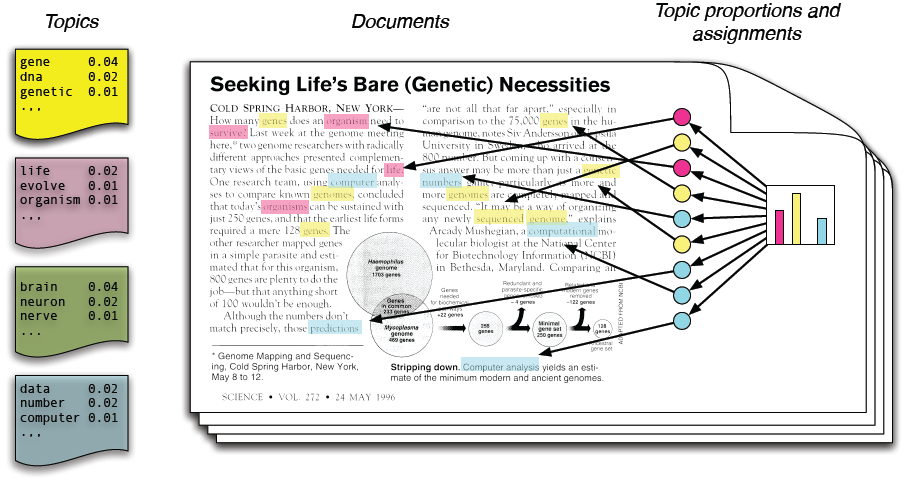
\includegraphics[width=1\linewidth]{figures/diagrama_lda}
	Fonte: \citeonline{rain2015lda}
\end{figure}

Na Figura 4 é possível visualizar um diagrama do processo generativo de palavras, sua correspondência com os tópicos e proporção nos documentos proposto por \citeonline{rain2015lda}. No exemplo do autor, LDA está utilizado para classificar tópicos em um artigo sobre ``evolução e o uso de análise de dados para determinar o número de genes que um organismo necessita para sobreviver''. Apesar de cada tópico não possuir valência como uma dimensão adjacente, uma analogia como a aplicação que propõem-se é utilizá-los como um indicador de temas. Basedo na proporção de termos, ao primeiro parágrafo, imputa-se o tema vermelho, ao segundo, amarelo e ao terceiro, azul. 

Com relação a quantidade de temas estimados, a literatura que lida com análise de tópicos com textos de discursos políticos varia na adoção de 8 até 500 componentes \cite{chen2010opinion, fang2012mining, balasubramanyan2012modeling, balasubramanyan2012modeling, cohen2013classifying, song2014analyzing, levy2014driving, van2014lda,zirn2014multidimensional}. Porém, as investigações que optaram por menor número de parâmetros obtiveram, em média, resultados mais verossíveis, ou passo que a identificação de muitos tópicos implicou em perda de similitude com codificações manuais. Assim, optou-se pela estimativa de 12 tópicos e do uso dos top 20 termos de cada um deles para codificação dos parágrafos. Conforme especificado na Equação 3.1, a polaridade de cada tópico é mensurada a partir da valência das sentenças dos parâgrafos que o compõem.  
 
\begin{figure}[h]
	\caption{Diagrama da Operacionalização das Estimações}
	\label{fig:diagram_op}
	\centering
	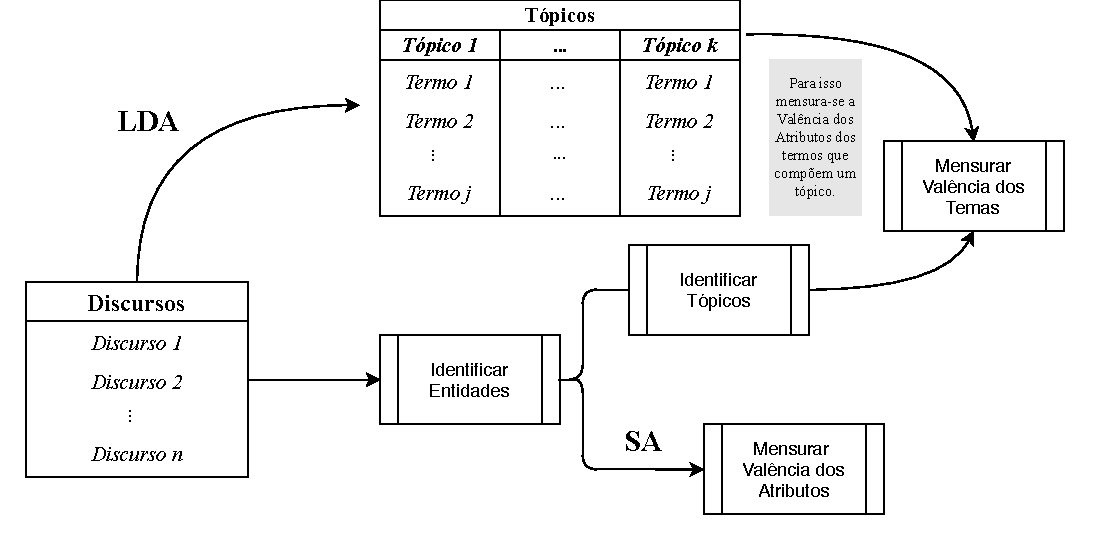
\includegraphics[width=1\linewidth]{figures/diagrama_operacionalizacao}
	Fonte: elaboração do autor
\end{figure}
 
Na Figura 6 é possível visualizar o diagrama do processo de estimação dos parâmetros do estimador de RWA proposto. De maneira sintética, utiliza-se LDA  -- tomando todo o escopo de textos da base da de dados -- para mapear as principais palavras que compõem cada um dos tópicos que segmentam os discursos políticos. Assume-se que cada tópico implica em um tema, que temas ocorrêm no nível de parágrafo. Para identificar afeição ou rejeição aos Valores Autoritários, primeiro, observa-se cada conjunto de discursos de um orador que contém alguma das Raízes do Quadro 1. A partir da seleção, a Valência da sentença em que a Raíz da Entidade ocorre é mensurada, o Tema no qual está inserida é detectado, tal como sua Valência, e assim é possível realizar a soma ponderada ilustrada pela Equação 3.3.

\chapter{Prova de Conceito: o caso da Câmara dos Deputados}\label{resultados}

\section{Introdução}

A combinação de um passado autoritário recente, um resultado eleitoral que levou a presidência um candidato com plataforma de campanha fortemente marcada por traços iliberais \cite{hunter2019bolsonaro} e um sistema político de grandes dimensões tornam o Brasil um candidato para a investigação da expressão de autoritarismo em grandes grupos.

Ao longo dos últimos anos, representantes políticos que estabelecem identidade de campanha baseada na memória do regime militar ou no passado profissional como membros das forças de repressão do Estado têm angariado cada vez mais espaço nos pleitos eleitorais \cite{berlatto2015candidatos, berlatto2016policia}. A trajetória de crescimento do seu desempenho é precipitada ainda por eventos que aumentam a saliência da questão de segurança, como os ataques do PCC em 2006. Consistente oposição aos direitos humanos, filiação a partidos pequenos, defesa combativa do crime e enrijecimento das formas de controle social são elementos característicos do conteúdo da sua atuação \cite{berlatto2015candidatos, berlatto2016policia, faganellobancada, faganello2017voto}

Do ponto de vista das tentativas de identificação do fenômeno, a literatura angaria uma variedade de critérios de classificação que captam, em maior ou menor medida, traços autoritários típicos de alguns grupos de representantes. Candidatos das Forças de Repressão do Estado e Políticos das Forças de Segurança são duas tipologias utilizadas para identificar, entre candidatos e parlamentares, aqueles indivíduos que estão comprometidos com a narrativa de corporações militares e policiais \cite{berlatto2015candidatos,berlatto2016policia}. Já a Bancada da Bala refere-se a uma agremiação informal de parlamentares que fazem \textit{lobby} para indústria armamentista e tendem a compor um conjunto de forças conservadoras nas câmaras estaduais e federal \cite{faganellobancada,faganello2017voto}.

Em um espectro próximo, há trabalhos que utilizam discursos de candidatos e parlamentares como fonte para fazer inferências sobre posicionamentos relativos à direitos reprodutivos \cite{miguel2017direito, santos2017debate}, sexualidade \cite{machado2013discursos, lacerda2016ideologia} e religiosidade \cite{gonccalves2016discurso}. Nessas investigações, conclusões acerca dos valores de tolerência e republicanismo adjacentes as falas compõem um mapa em formação das atitudes democráticas entre os representantes políticos. Contudo, nem todos os Políticos das Forças de Segurança, Candidatos das Forças de Repressão do Estado ou da Bancada da Bala se opõem aos princípios democráticos, por vezes se limitam ao comportamento corporativista. Além disso, uma observação segmentada das falas impede a construção de índices de preconceito generalizado. 

Nas seções a seguir, serão detalhados os passos da construção de indicadores de RWA para os parlamentares brasileiros, a partir de suas falas, conforme os pressupostos e especificações definidas nas seções anteriores.

\section{Coletando e Organizando Dados}

Como forma de ampliar a transparência entre as atividades do plenário e os cidadãos, a Câmara dos Deputados possui o serviço de Dados Abertos, que conta com uma API de consulta pública, possibilitando a extração de dados de Blocos, Deputados, Eventos, Frentes, Legislaturas, Partidos, Proposições, Referências, Votações e Órgãos. A iniciativa, lançada em 2017 em consonância com a Lei de Acesso à Informação de 2011, permite o acesso fácil e o consumo em larga escala dos produtos do trabalho de transcrição e catalogação do Regimento Interno da Câmara dos Deputados.

No que diz respeito a velocidade de coleta, a documentação da API consta que, no período de 6:00 às 23:59, o Portal aceita 90 requisições por minuto e, das 00:00 às 5:59, 300. Foi por meio da API que os grandes volumes de dados de discursos de parlamentares foram extraídos de forma otimizada, utilizando \emph{framework} de raspagem de dados assíncrona. No período de elaboração dessa dissertação, as transcrições dos discursos realizados no plenário estavam disponíveis a partir dos anos 2000. Com isso, foi possível processar as falas proferidas entre a segunda metade da 51ª legislatura e meados da 56ª, permitindo a observação longitudinal de mais de 20 anos de atividade da Câmara dos Deputados, identificando de traços atitudinais em oradores que se manifestaram em pelo menos uma das seções.

\begin{center}
	Tabela 2 - Estatísticas de Oradores por Legislatura
	
	\vspace{0.4cm}
	
	\begin{tabular}{lccccccc}
		\toprule
		{}				& {51*}		& {52} 	& {53}	& {54}	& {55}	& {56**}	& {Total}	\\ \midrule
		{Deputados} 	& 642		& 629	& 646	& 671	& 633	& 545		& 3766		\\ 
		{Oradores} 		& 614		& 604	& 595	& 631	& 604	& 508		& 3556		\\ \midrule
		{Discursos} 	& 31377		& 77458	& 83629	& 83468	& 88265	& 24974		& 389171	\\ 
		\bottomrule
	\end{tabular}
	
	\vspace{0.6cm}
	
	* : dados coletados a partir de Janeiro de 2000; ** : dados coletados até Maio de 2020.
\end{center}

Na Tabela 2 é possível observar, em cada uma das legislaturas, o número de Deputados ativos -- contanto com eleitos e suplentes que assumiram o mandato em algum momento -- o número de Oradores -- Deputados ativos que realizaram ao menos algum discurso em alguma das seções -- e o volume de Discursos realizados. Descartando as legislaturas 51 e 56, por apresentarem dados restritos, é possível observar um movimento de crescimento da quantidade de discursos que não é acompanhado pelas flutuações no número de oradores. No total, ao longo do perído de coleta, 389.171 discursos foram realizados por 3556 parlamentares\footnote{É importante ressaltar que, seguindo a estratégia metodológica de \citeonline{moreira2016palavra}, são considerados registros multíplos em caso de indivíduos que foram eleitos para legislaturas distintas. Ou seja, um parlamentar é contado uma vez por legislatura para qual elegeu-se.}.

\begin{figure}[h]
	\caption{Quantis da Frequência de Realização de Discursos por Legislatura}
	\label{fig:quantis_discursos}
	\centering
	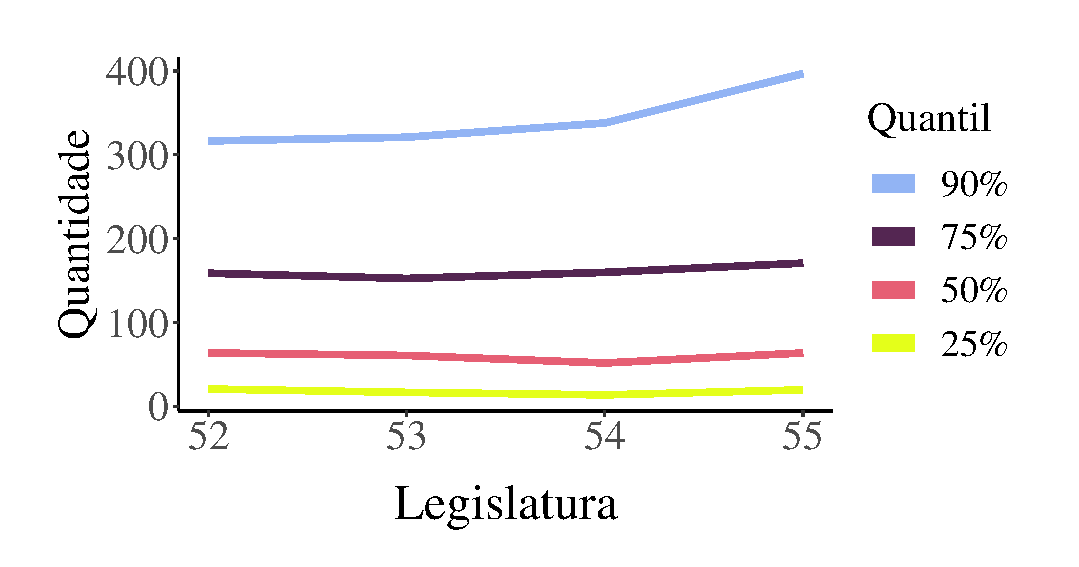
\includegraphics[width=.7\linewidth]{figures/quantis_discursos}
	
	Fonte: elaboração do autor
\end{figure}

Ainda no que diz respeito a tendência de ampliação do uso do espaço de fala, a Tabela 2 oferece indícios para inferir que esse processo decorre da concentração de pronunciamentos em uma porção restrita de parlamentares. A despeito das flutuações nos valores da mediana, os quantis mais elevados de frequência têm seus valores ampliados ao longo da série histórica. Essa dinâmica acentua um fato documentado pela literatura, e reforçado pela Figura 8, de que uma minoria de Deputados concentra grande espaço nos pronunciamentos do plenário \cite{moreira2016palavra}. Em todas as legislatura, é possível identificar uma distribuição de hiper-concentrada nos valores mais baixos e uma longa calda onde estão incluídos os palamentares mais comunicativos.    

\begin{figure}[!htb]
	\caption{Distribuição da Realização de Discursos por Legislatura}
	\centering
	
	\begin{minipage}[b]{0.3\textwidth}
	\textbf{Legislatura 51}
	\label{fig:dens_legis_51}
	\centering
	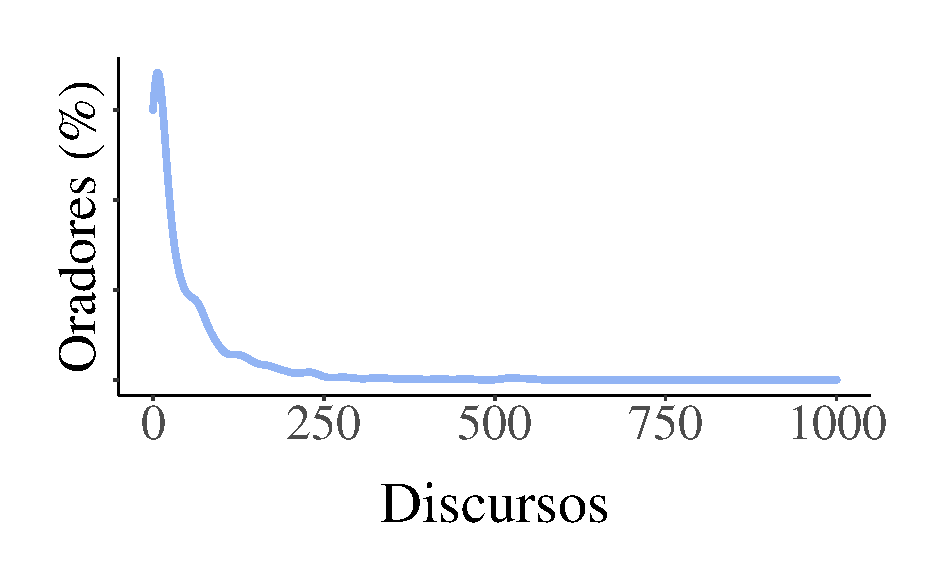
\includegraphics[width=1\linewidth]{figures/dens_oradores_51}
	
	\end{minipage}
	\hspace{.05\linewidth}
	\begin{minipage}[b]{0.3\textwidth}
		\textbf{Legislatura 52}
		\label{fig:dens_legis_52}
		\centering
		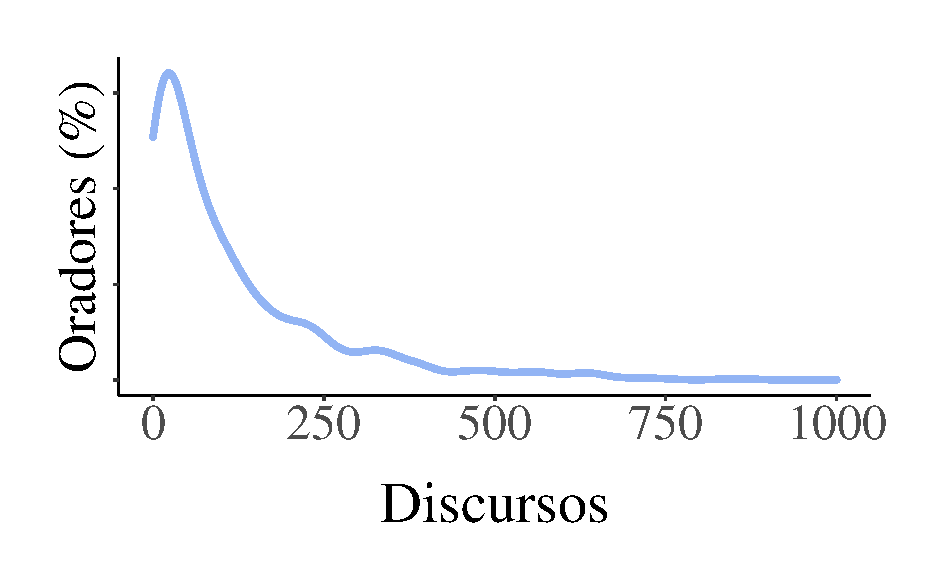
\includegraphics[width=1\linewidth]{figures/dens_oradores_52}
		
	\end{minipage}
	\\
	\hspace{.05\linewidth}
	\begin{minipage}[b]{0.3\textwidth}
		\textbf{Legislautra 53}
		\label{fig:dens_legis_53}
		\centering
		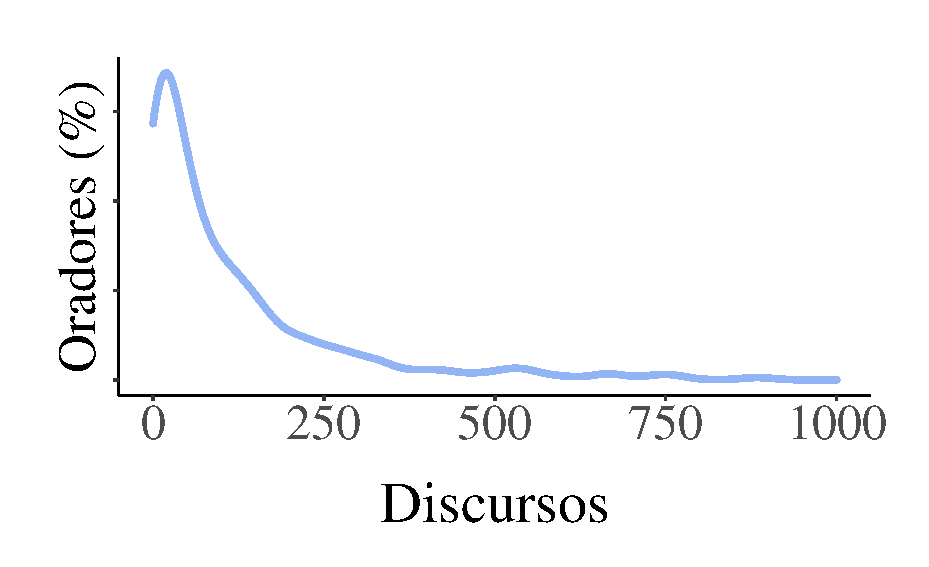
\includegraphics[width=1\linewidth]{figures/dens_oradores_53}
		
	\end{minipage}
	\hspace{.05\linewidth}
	\begin{minipage}[b]{0.3\textwidth}
		\textbf{Lgislatura 54}
		\label{fig:dens_legis_54}
		\centering
		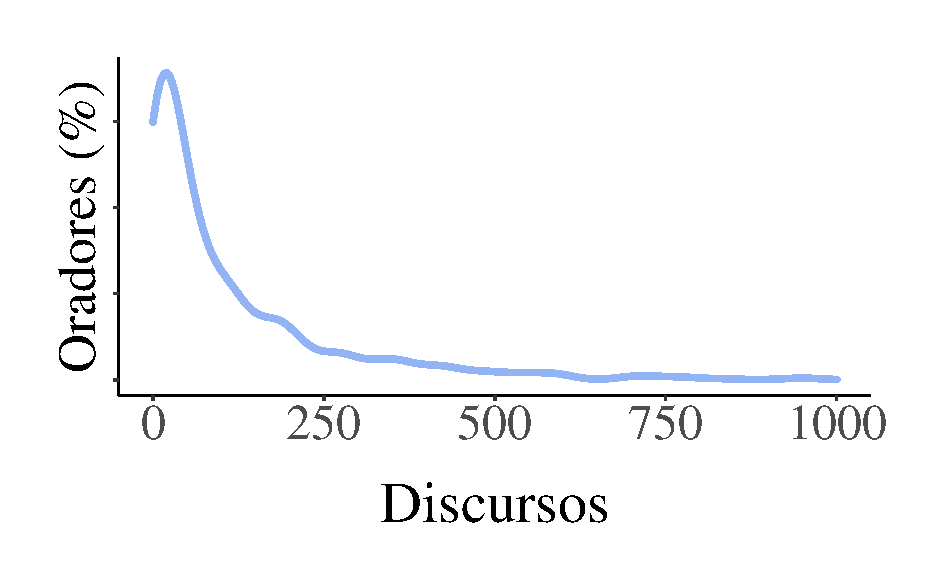
\includegraphics[width=1\linewidth]{figures/dens_oradores_54}
		
	\end{minipage}
	\\
	\hspace{.05\linewidth}
	\begin{minipage}[b]{0.3\textwidth}
		\textbf{Legislautra 55}
		\label{fig:dens_legis_55}
		\centering
		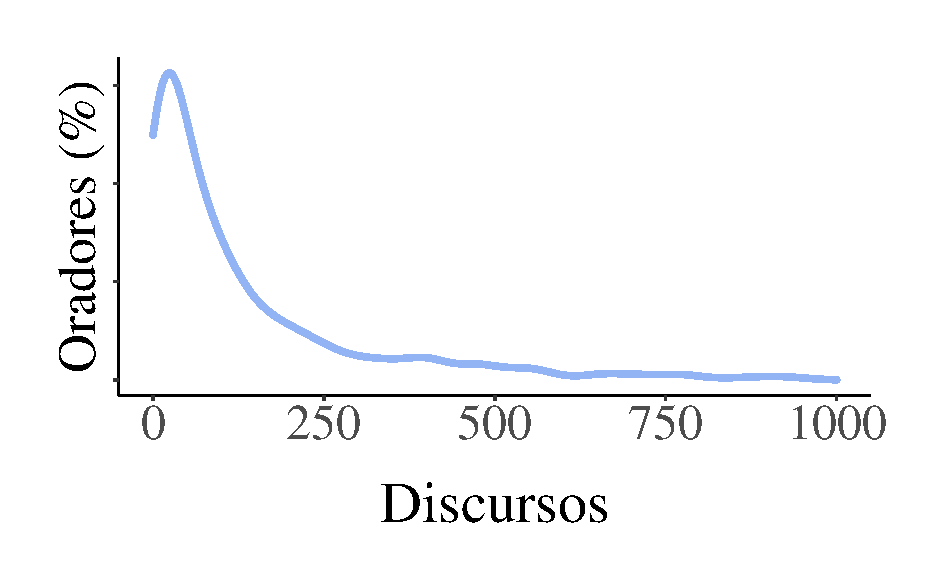
\includegraphics[width=1\linewidth]{figures/dens_oradores_55}
		
	\end{minipage}
	\hspace{.05\linewidth}
	\begin{minipage}[b]{0.3\textwidth}
		\textbf{Legislatura 56}
		\label{fig:dens_legis_56}
		\centering
		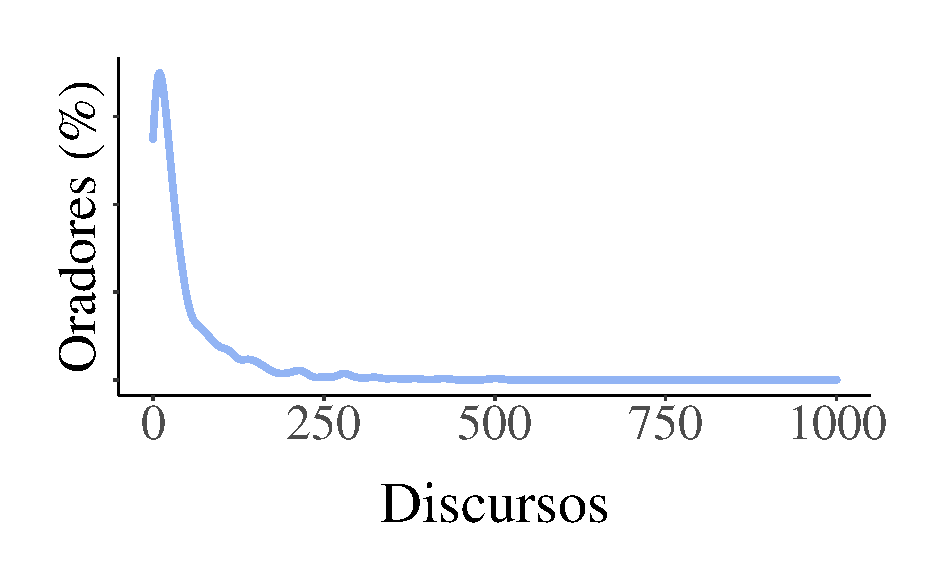
\includegraphics[width=1\linewidth]{figures/dens_oradores_56}
		
	\end{minipage}	

	Fonte: elaboração do autor
	\begin{flushleft}
		Nota: O limite das abcissas dos gráficos foi fixado com o propósito de facilitar a visualização. Os pontos de máximo para as legislaturas são: 1186, 51; 2383, 52; 5965, 53; 2268, 54; 1829, 55 e 501, 56. 
	\end{flushleft} 
\end{figure}

Além de observar a frequência de pronunciamentos parlamentares, para a estimação do indicador de RWA proposto, é necessário observar a ocorrência de raízes de palavras que mapeiam cada uma das dimensões do autoritarismo, conforme foi especificado no Quadro 1. Na Figura 9 é possível observar que a ocorrência de termos pertencentes a cada dimensão segue o padrão de distribuição concentrada nos valores mais baixos e esparsa nos mais altos. É importante ressaltar que o gráfico não representa os valores de Submissão à Autoridade, Agressividade Autoritária e Convencionalismo em si, mas a ocorrência de termos que tornam possível estimar o posicionamento latente do parlamentar em relação aos Valores Autoritários.

\begin{figure}[h]
	\caption{Distribuição da Ocorrência de Raízes das Dimensões de RWA}
	\label{fig:dens_ocorrencia_termos}
	\centering
	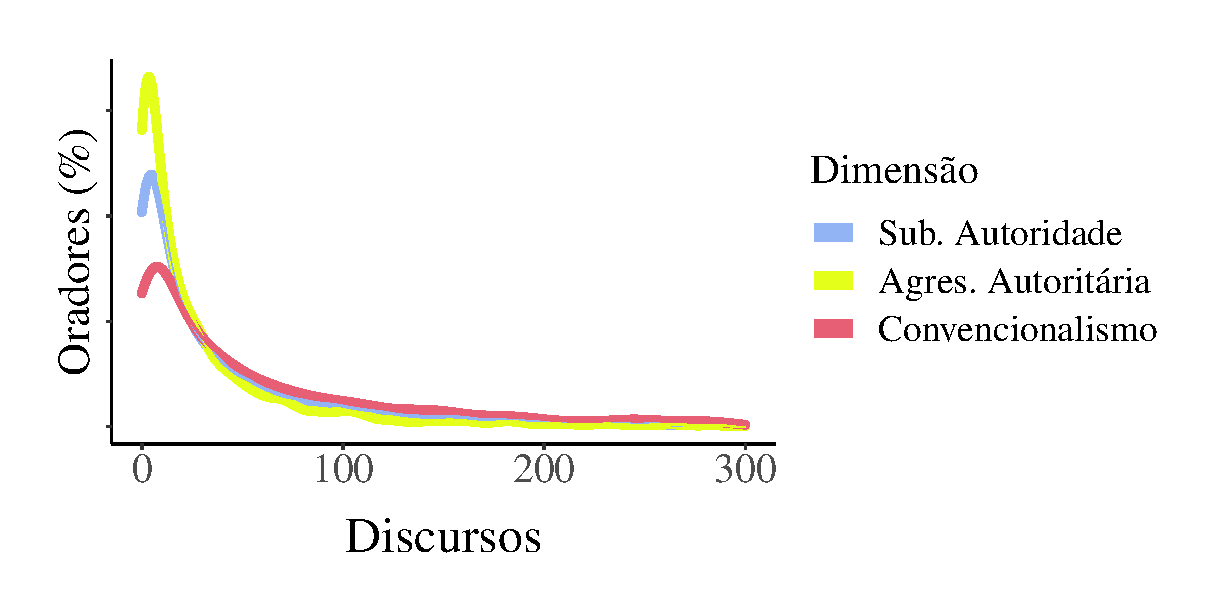
\includegraphics[width=.7\linewidth]{figures/dens_dimensoes_rwa}
	
	Fonte: elaboração do autor
	\begin{flushleft}
	Nota: O limite da abcissa do gráfico foi fixado com o propósito de facilitar a visualização. Os pontos de máximo para as dimensões do RWA são: 2597, Submissão à Autoridade; 2001, Agressividade Autoritáriae e 4437, Convencionalismo. 
	\end{flushleft} 	
\end{figure}

Ainda sobre a Figura 9, pode-se inferir que ocorrência de termos pertencentes a uma dimensão do autoritarismo é maior quando a cauda da sua distribuição é mais pesada. Nesse sentido, é possível identificar mais discursos em que parlamentares manifestaram adesão ou rejeição a valores Convencionalistas do que de à Submissão à Autoridade e à Agressividade Autoritária. Ao todo, ao longo de todas as legislaturas, 3475 parlamentares mencionaram alguma Entidade referente a Convencionalismo, 3386, referente à Submissão à Autoridade e 3335, referente à Agressividade Autoritária. Esses números indicam que a Tipologia de Entidades definina possui grande cobertura e, consequentemente, permite uma estimativa parcial da Escala de Valores Autoritários para uma parte substancial dos Deputados.

Na seção seguinte, serão apresentados os procedimentos para estimativa de RWA entre parlamentares brasileiros a partir dos seus pronunciamentos no plenário da Câmara dos Deputados.

\section{Estimando RWA entre Deputados}


\section{Avaliando resultados}

aa
% ----------------------------------------------------------
% ELEMENTOS PÓS-TEXTUAIS
% ----------------------------------------------------------
\postextual
% ----------------------------------------------------------

% ----------------------------------------------------------
% Referências bibliográficas
% ----------------------------------------------------------
\bibliography{bibli}

% ----------------------------------------------------------
% Glossário
% ----------------------------------------------------------
%
% Consulte o manual da classe abntex2 para orientações sobre o glossário.
%
%\glossary

% ----------------------------------------------------------
% Apêndices
% ----------------------------------------------------------

Apêndices

%---------------------------------------------------------------------
% INDICE REMISSIVO
%---------------------------------------------------------------------
\phantompart
\printindex
%---------------------------------------------------------------------

\end{document}
